\chapter{Research Methods}
\label{cha:methods}
\acresetall

The previous chapter gave an overview of the research done in affect detection, \gls{behaviomedics}, and multimodal data fusion. Based on the state-of-the-art, the goal is to create a multimodal framework to analyze the relationship of emotions, expressed emotions, and speech errors. For that purpose, experts need to be consulted in order to gain more insights of motoric speech disorders and to have access to patients. In chapter~\ref{sec:experts} institutions are listed which can be approached for that matter. Whilst contact is built with the experts, available datasets shown in chapter~\ref{subsec:availableData} can be used to build a multimodal framework. In chapter~\ref{subsec:collectedData} collected data of 67 children will be described, as well as the risen challenges to analyze the data.
Subsequent the creation of a new multimodal dataset of exercises performed by \gls{pws} or patients with \gls{pd} or \gls{ad} suffering \gls{apraxia} or \gls{dysarthria} is described. 
The chapter ends with an overview of sensors which can be used for data collection and the features which can be used in each modality. 

\section{Expertise Consulting}
\label{sec:experts}
As the proposed project is interdisciplinary, it is necessary to create contacts to medical centers where expertise about \gls{stuttering}, \gls{dysarthria} and \gls{apraxia} caused by underlying neurodegenerative diseases can be found.

Expertise in dysfluency can be found at the \textbf{Stuttering Center of Western Pennsylvania} which is located in Pittsburgh. It works in collaboration with the Department of Audiology and Speech-Language Pathology at Children's Hospital of Pittsburgh of \gls{upmc} and the Department of Communication Science and Disorders at the University of Pittsburgh. It is an institution which is open to research concerning stuttering. 
%Dr. J. Scott Yaruss, Director of the Stuttering Center, is the responsable contact for research cooperations (jsyaruss@pitt.edu).

At the \textbf{\gls{upmc} Voice Center} voice disorders are evaluated and treated for both the general public and those who use their voices professionally. One of the therapies which are provided is the "Lee Silverman Voice Treatment". It is a proven speech treatment program for people with \gls{pd}. It helps restore oral communication beyond what current medicines and surgical interventions can offer. At the UPMC Voice Center, a modified version of this program is provided, focusing on increasing vocal loudness, enhancing sensory awareness of disordered movement parameters, and "re-calibrating" the sensorimotor system for appropriate movement dynamics.
The UPMC Voice Center also participates in several research studies such as in "defining the Minimal Clinically Important Difference of the Voice Handicap Index-10". The goal of this study is to find out how a change in patient-perceived voice handicap correlates with clinical improvement in voice. 

Additional information can be obtained from the \textbf{Department of Neurology of the University of Pittsburgh}, where several neurodegenerative diseases causing movement disorders are treated \footnote{
\url{http://www.neurology.upmc.edu/movement/}}. Furthermore, it has been designated by the American Parkinson Disease Association (APDA) \footnote{ \url{https://www.apdaparkinson.org}} as one of only eight Advanced Centers for Parkinson’s Disease Research in the nation.

\section{Datasets}

\subsection{Creation of Baseline with Available Multimodal Datasets}
\label{subsec:availableData}
Available datasets will be used to create baselines for emotion classification. The RECOLA multimodal corpus used in the AVEC 2016 emotion sub-challenge contains data of remote and collaborative affective interactions. It contains audio-visual and physiological data for emotion recognition. To create a multimodal baseline, toolboxes mentioned in \ref{sec:sensorsFeatures} will be used to create hand-crafted features. The features will be used for unimodal supervised classification as well as for data fusion and multimodal supervised classification.  The results can be evaluated using the F1-score, precision and recall.

As baseline to detect distress, anxiety and depression, the DAIC-WOZ database \footnote{ \url{http://dcapswoz.ict.usc.edu/wwwutil_files/DAICWOZDepression_Documentation.pdf}} from AVEC 2016 will be used. It contains clinical interviews designed to support the diagnosis of psychological distress conditions such as anxiety, depression, and post-traumatic stress disorder \cite{Valstar2016avec}. The same methods will be applied as for the first dataset.

The creation of a multimodal baseline using existing datasets has several advantages. Time is saved in data collection, several researchers used the datasets and results and methods are published, and implementation mistakes can be detected through comparison with the results of other researchers.


\subsection{Collected Dataset}
\label{subsec:collectedData}
In October and November of 2016, preliminary recordings were performed using a Microsoft Kinect v2 to record 67 children between the ages of 7 -11 during the performance of oromotoric exercises. The recordings were performed in two different elementary schools in Lisbon, always in a room of the school (see setup in Fig.~\ref{fig:setup}). Children without any prior knowledge of detected speech or language disorders were recorded. The exercises were chosen by the \glspl{slp} shown in Fig.~\ref{fig:recordedEx} and were guided by 4 of them. In order to meet the anonymity requirements by the ethics committee, a black bar was placed over the eyes. 
The children had to perform each exercise in isolation and then performed rapid alternations between two exercises as can be seen in Fig.~\ref{fig:recordedSeq}.

Challenges in the data: 
\begin{itemize}
    \item \textbf{Unusual movements were difficult to perform:} Although the exercises were explained and demonstrated prior to execution, movements which involved lip movement to the sides as well as jaw movements were not always performed correctly. Haptic feedback was given by touching the cheek or the jaw to guide the movement direction, but was not always enough.
    \item \textbf{Order of the exercises was not fixed:} There are variations in the order of the exercises, as well as interruptions. Exercises needed to be interrupted as the children lost concentration as well as to talk to them and gain some trust. The order of the exercises was not always the same, which implies a manual labeling of the data for exercises, and removal of frames in which the \gls{slp} was talking to the child.
    \item \textbf{Variations in the explanation:} Explanation of exercises as well as how often it was repeated or how it was reformulated various in each \gls{slp}. 
    \item \textbf{Repetition frequency varies:} Some children repeated the exercises more often than others.
\end{itemize}
 The mentioned challenges difficult the analysis of the exercise performance. However, it can be used to test geometric feature detection in 3D data. 


\begin{figure}
    \centering
    \subbottom[Bird's view of the recording setup. ]{
    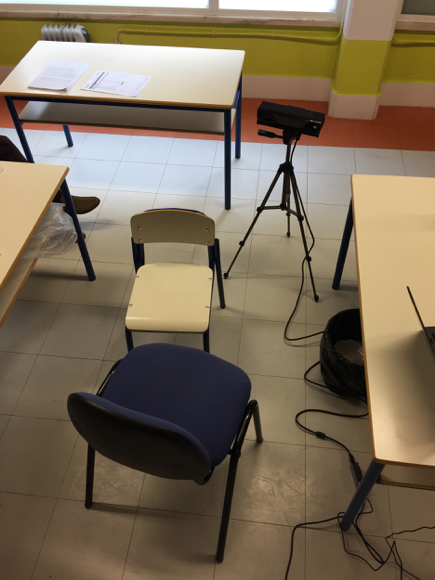
\includegraphics[height=6cm]{setup}}\hspace{0.5cm}
    \subbottom[Image recorded by the RGB camera of the Kinect with children in resting position.]{
    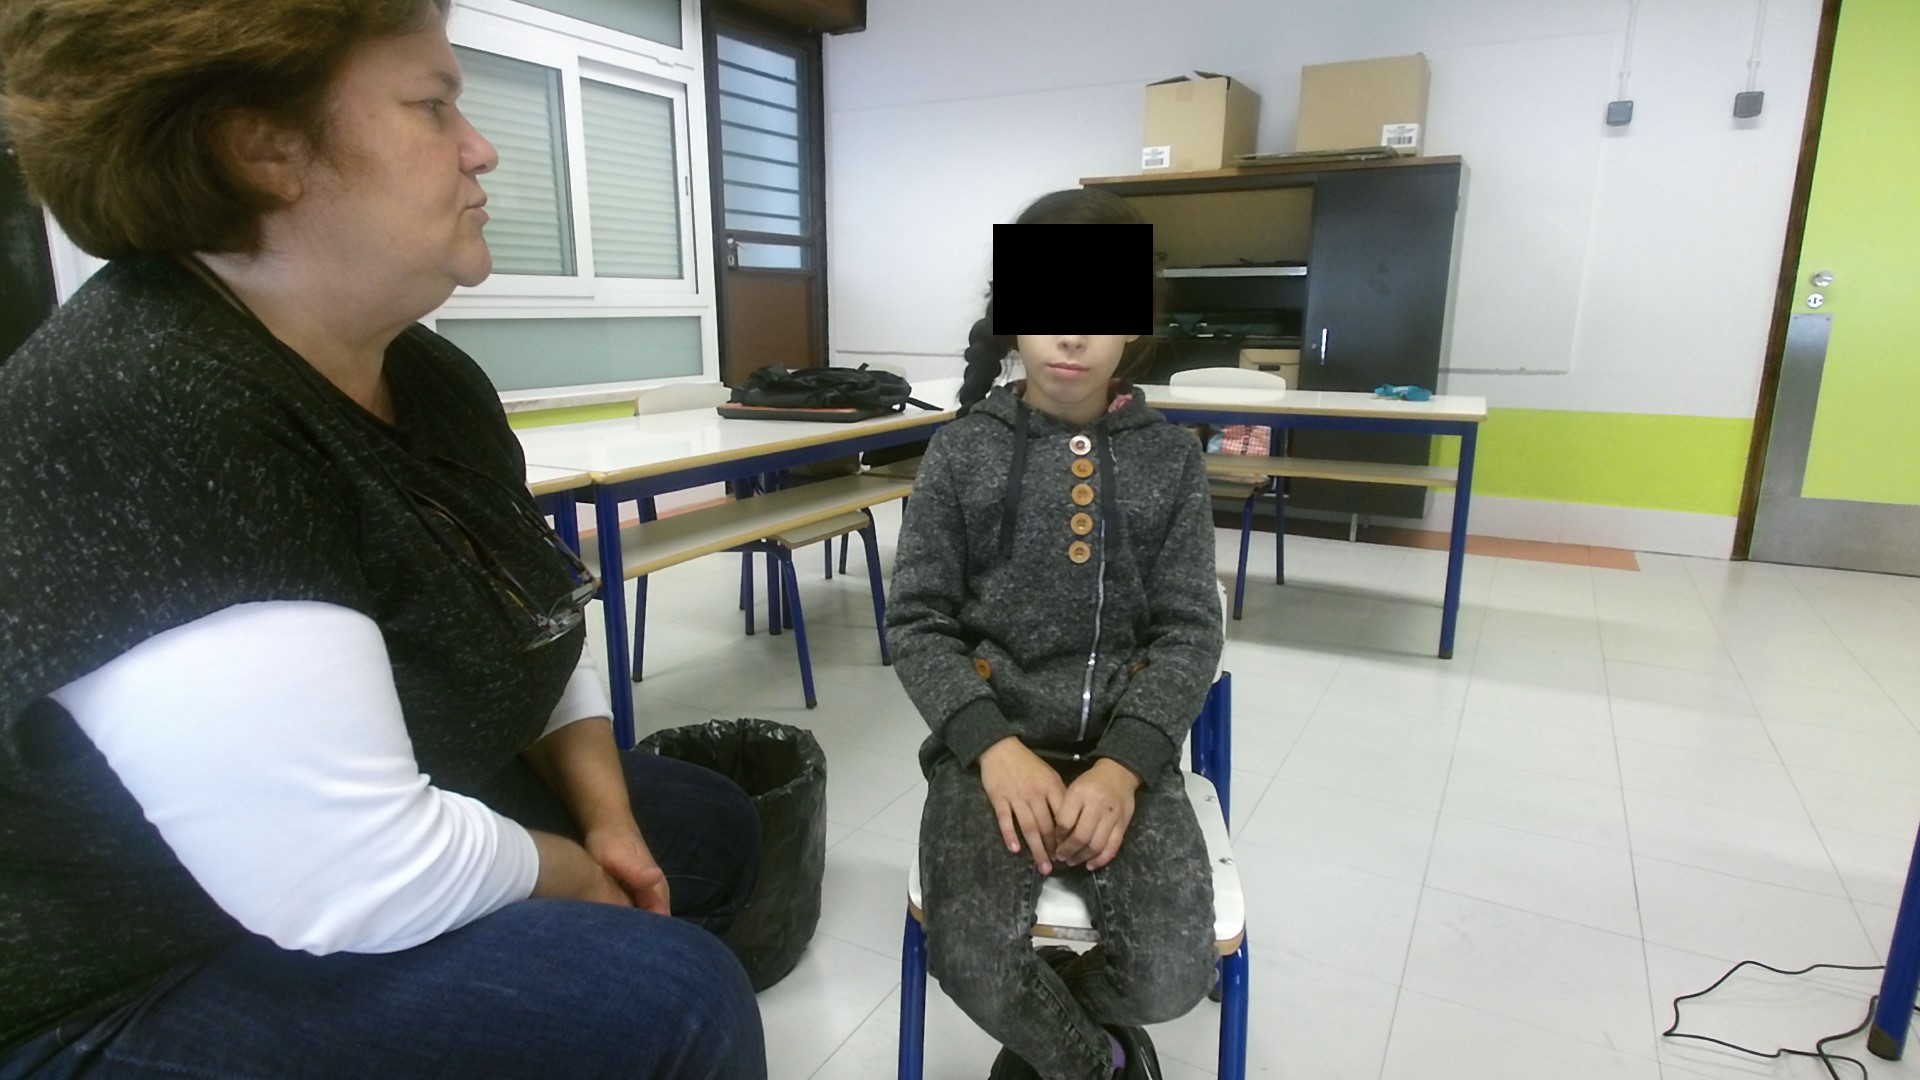
\includegraphics[height=6cm]{color_13_resting}}
    \caption{Setup of the recording done at an elementary school for screening of speech and language disorders and a RGB frame recorded with the Kinect 2.}
    \label{fig:setup}
\end{figure}

\begin{figure}[htbp]
\centering
 \subbottom[Lips protrusion.]{%
    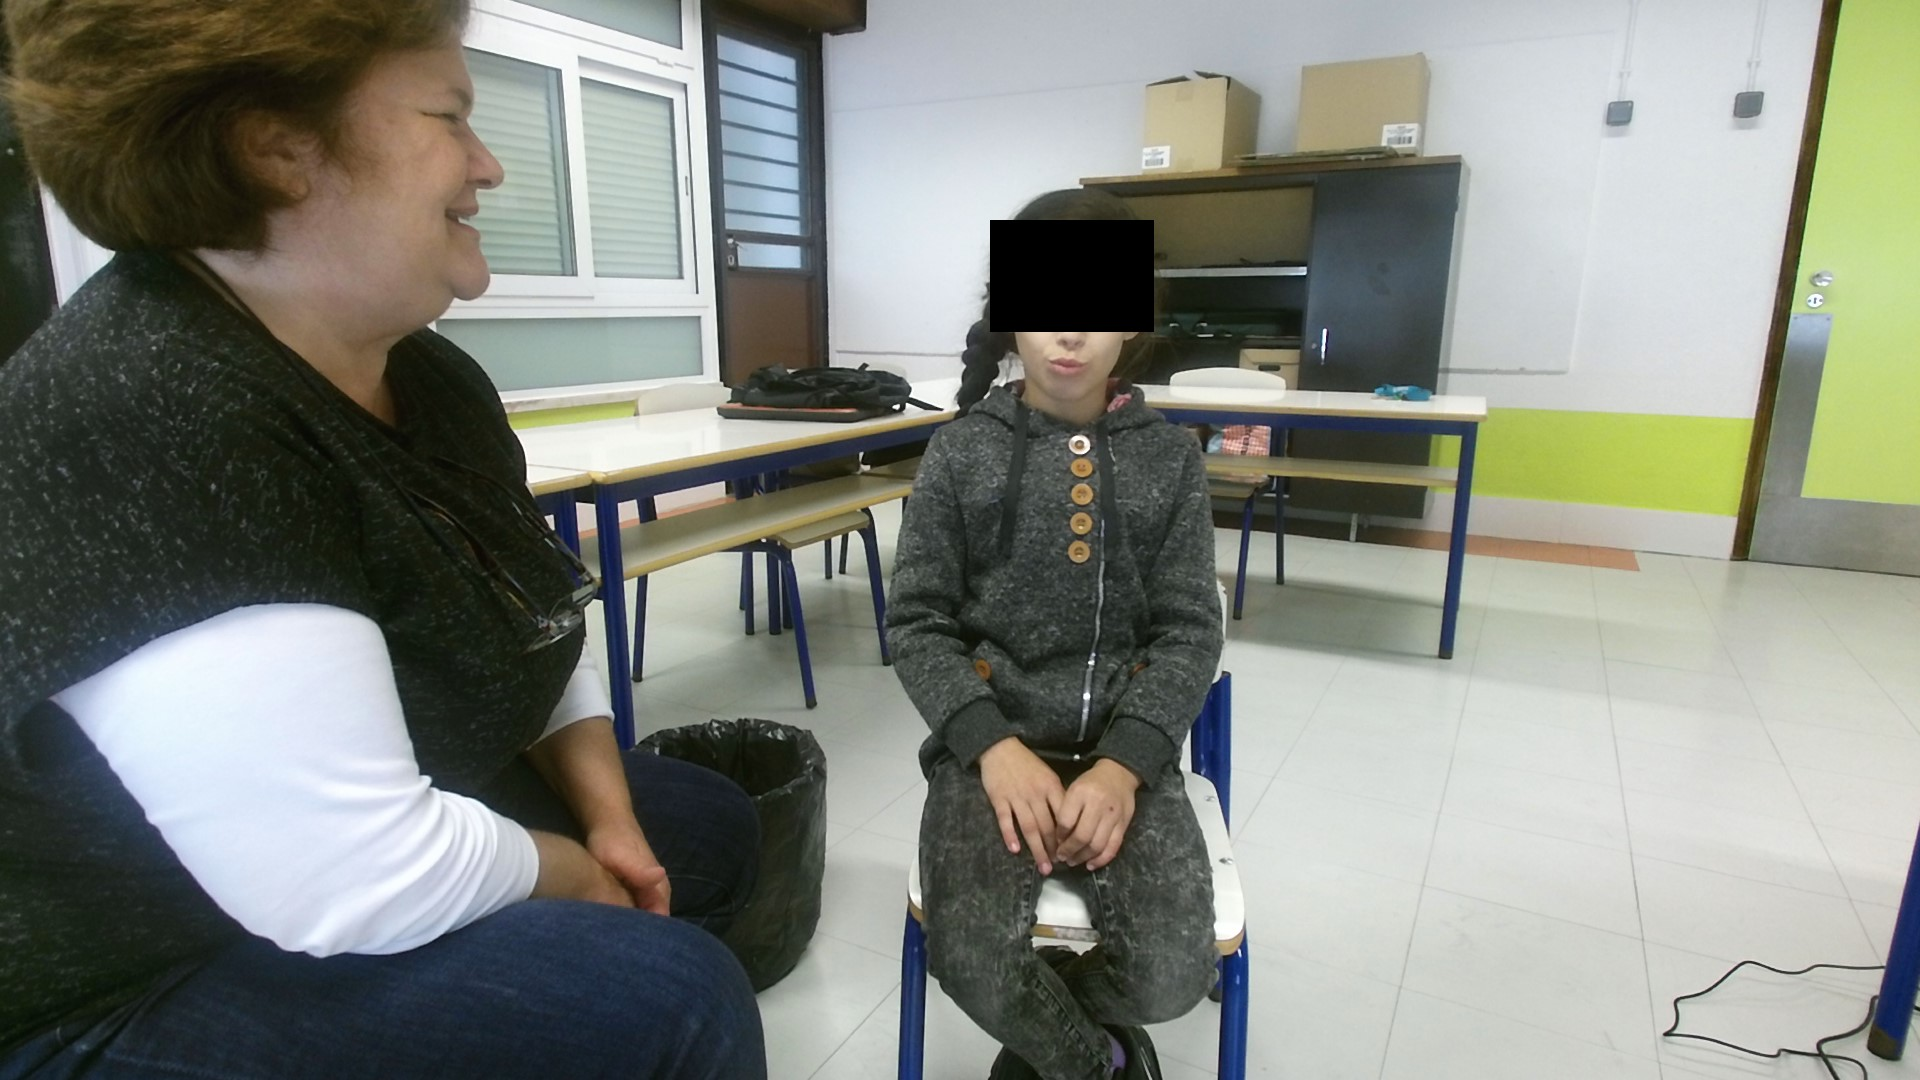
\includegraphics[trim=23cm 15cm 18cm 4cm, clip, width=0.3\linewidth]{color_14_protrusion}}%
 \subbottom[Smile]{%
    \hspace{0.3cm}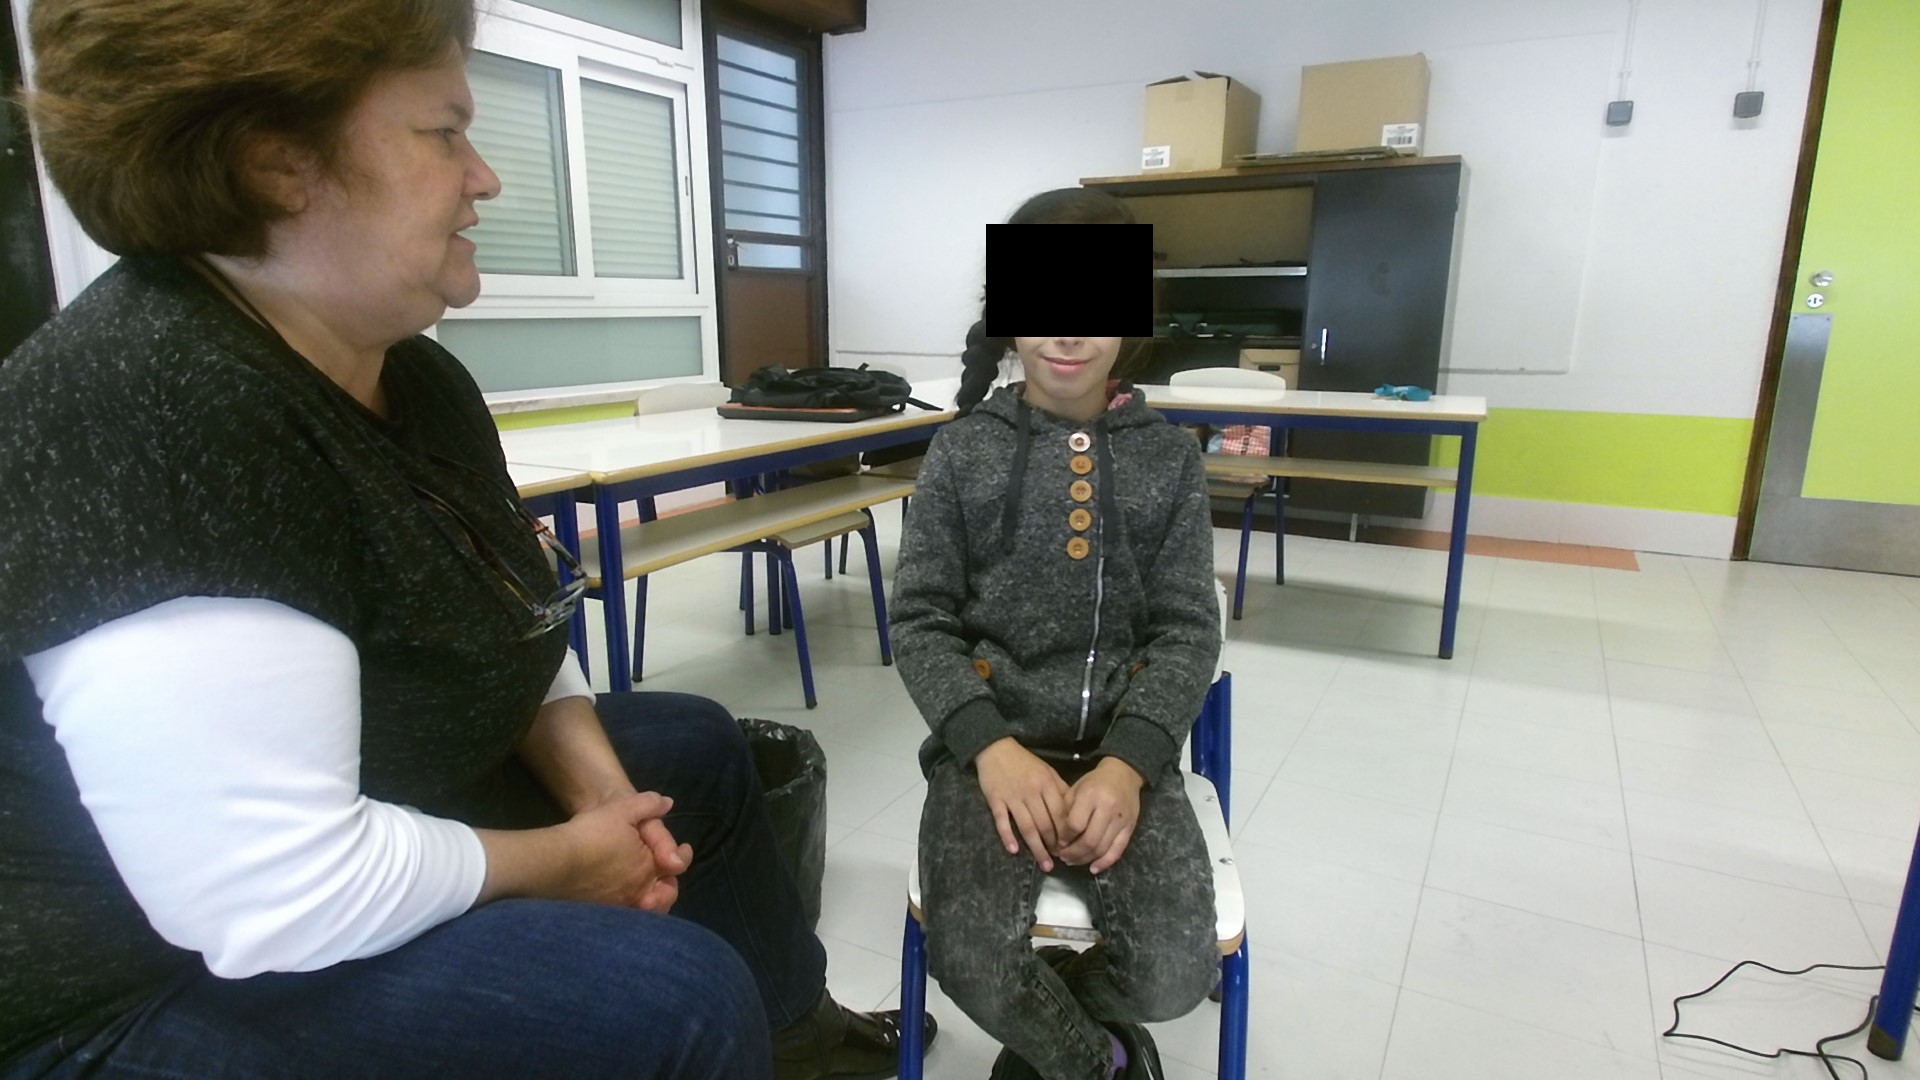
\includegraphics[trim=23cm 15cm 18cm 4cm, clip,width=0.3\linewidth]{color_46_smile}}
 \subbottom[Lips to the right.]{%
    \hspace{0.3cm}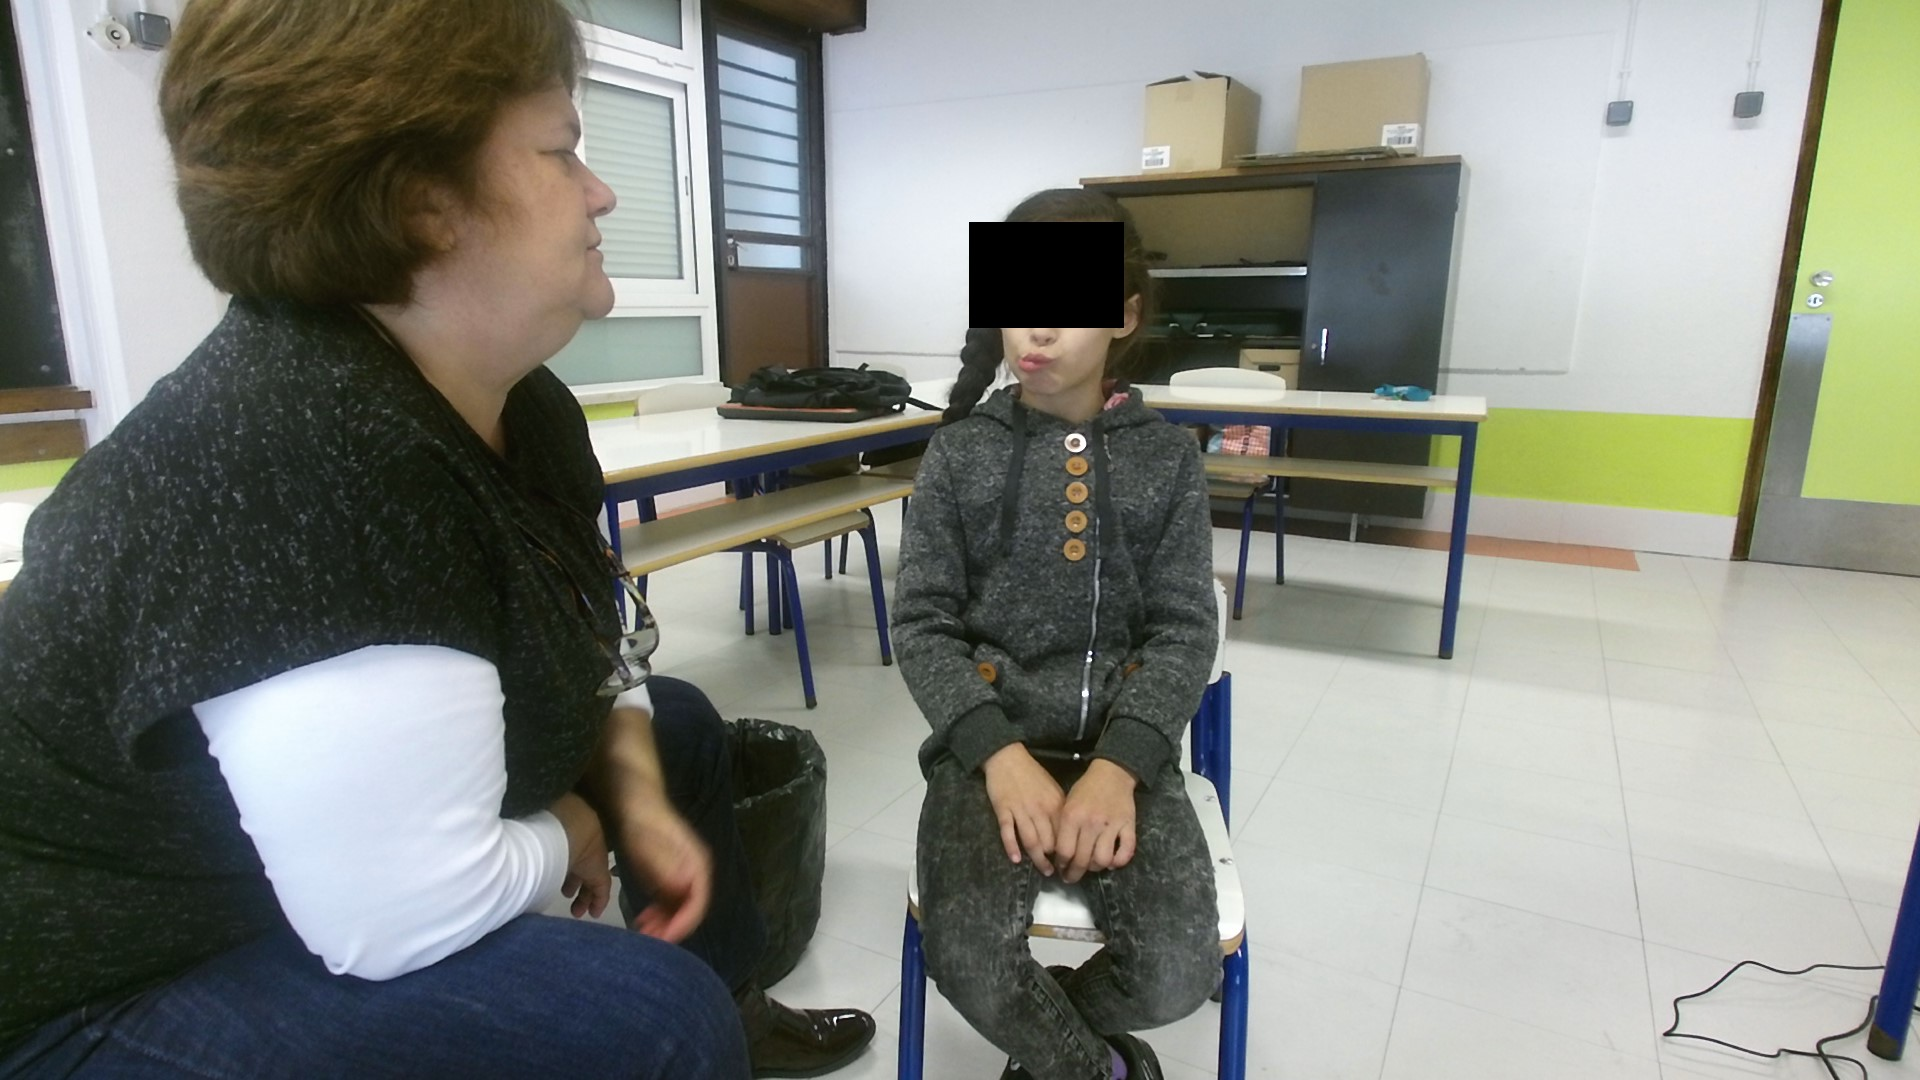
\includegraphics[trim=23cm 15cm 18cm 4cm, clip,width=0.3\linewidth]{color_261_lipstoright}}\\
    \subbottom[Lips to the left.]{%
    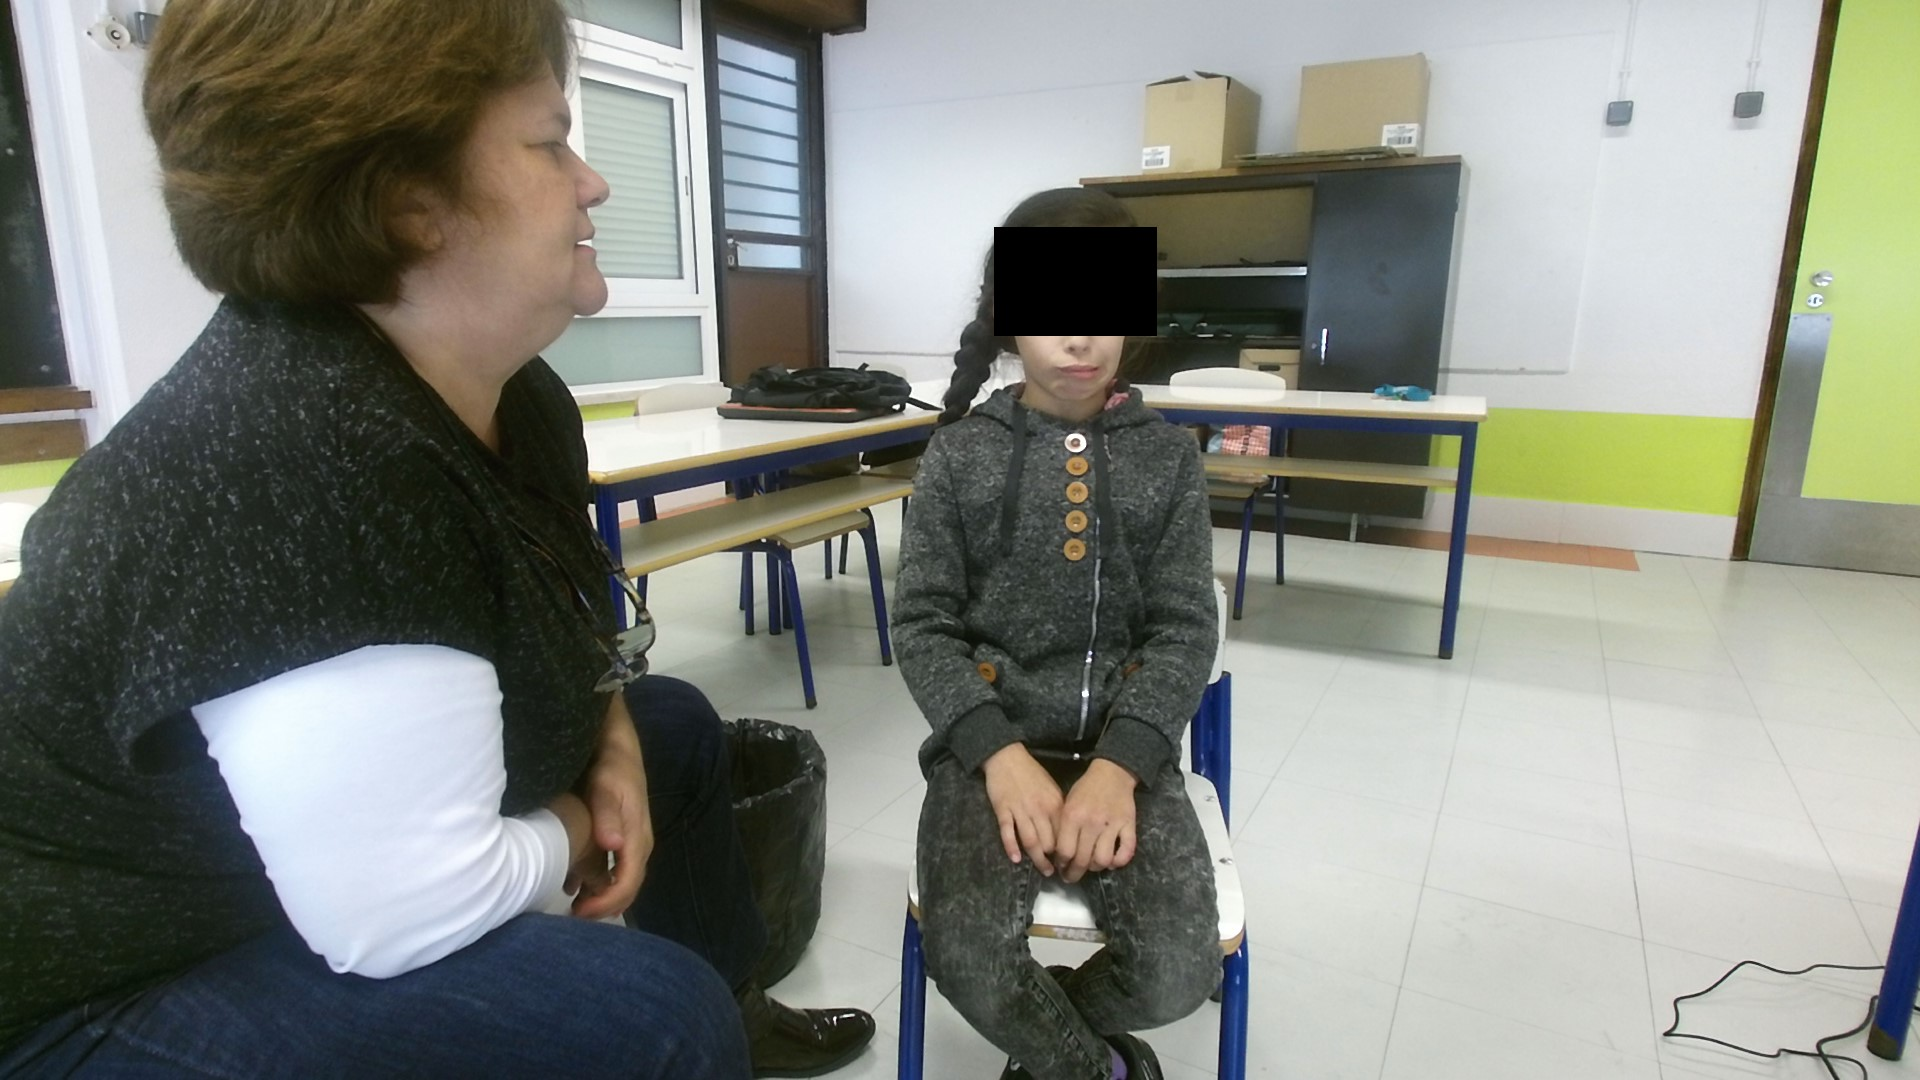
\includegraphics[trim=23cm 15cm 18cm 4cm, clip,width=0.3\linewidth]{color_266_lipstoleft}} 
 \subbottom[Opened mouth.]{%
    \hspace{0.3cm}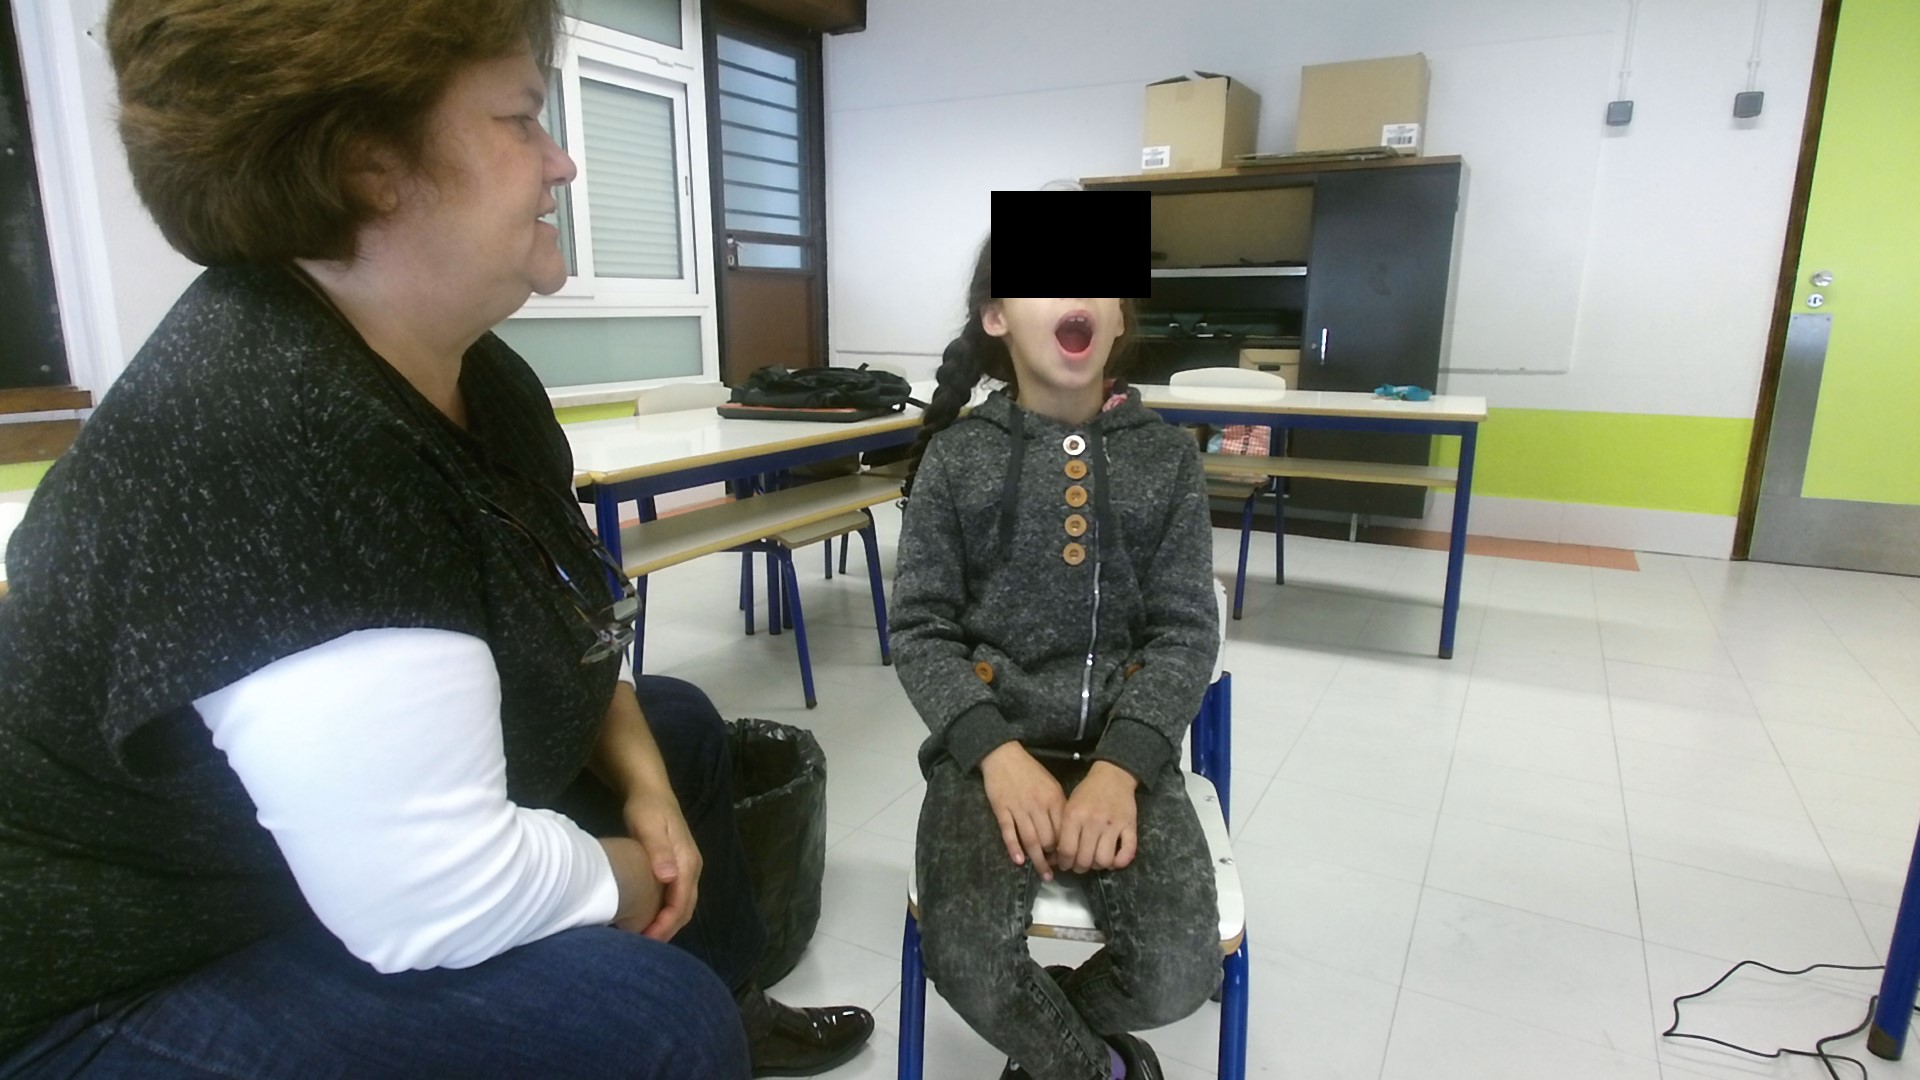
\includegraphics[trim=23cm 15cm 18cm 4cm, clip,width=0.3\linewidth]{color_342_openMouth}}    	
\subbottom[Closed mouth.]{%
    \hspace{0.3cm}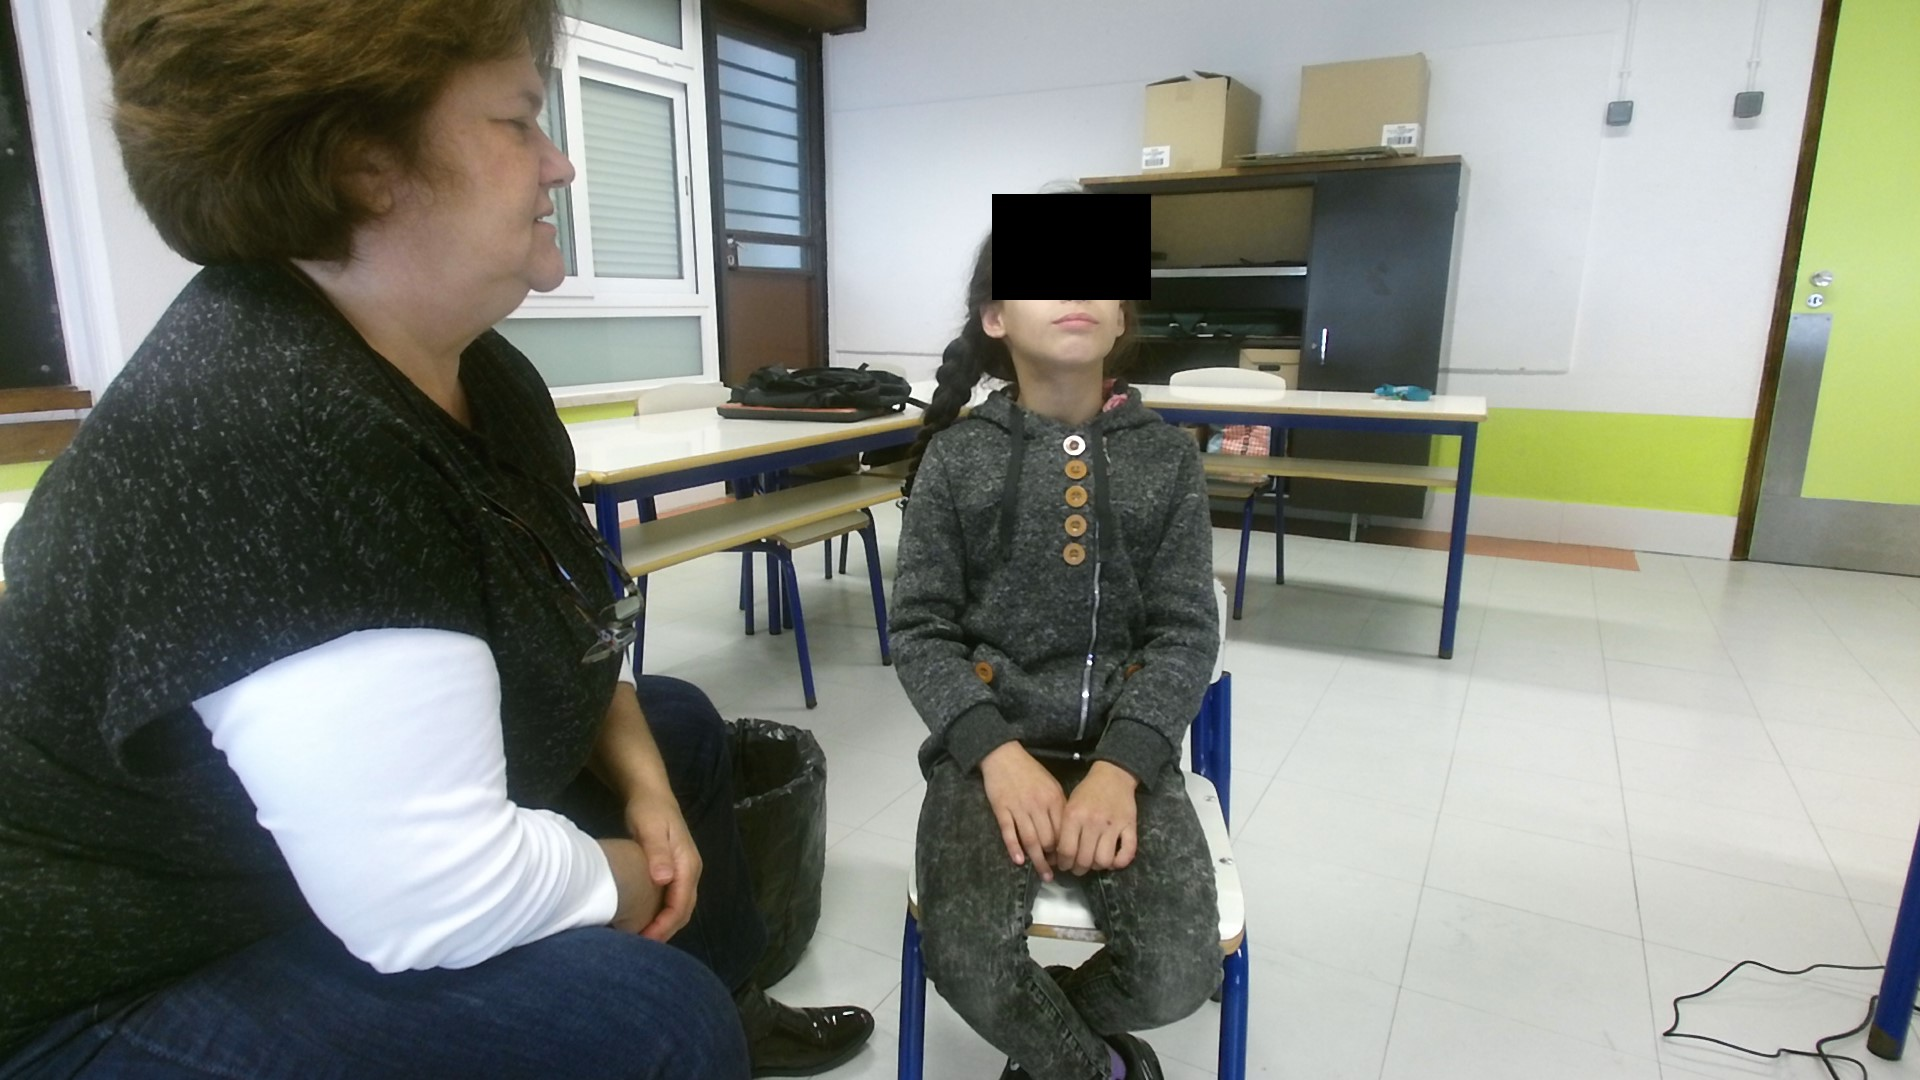
\includegraphics[trim=23cm 15cm 18cm 4cm, clip,width=0.3\linewidth]{color_343_closeMouth}}\\
 \subbottom[Jaw front.]{%
    \hspace{0.3cm}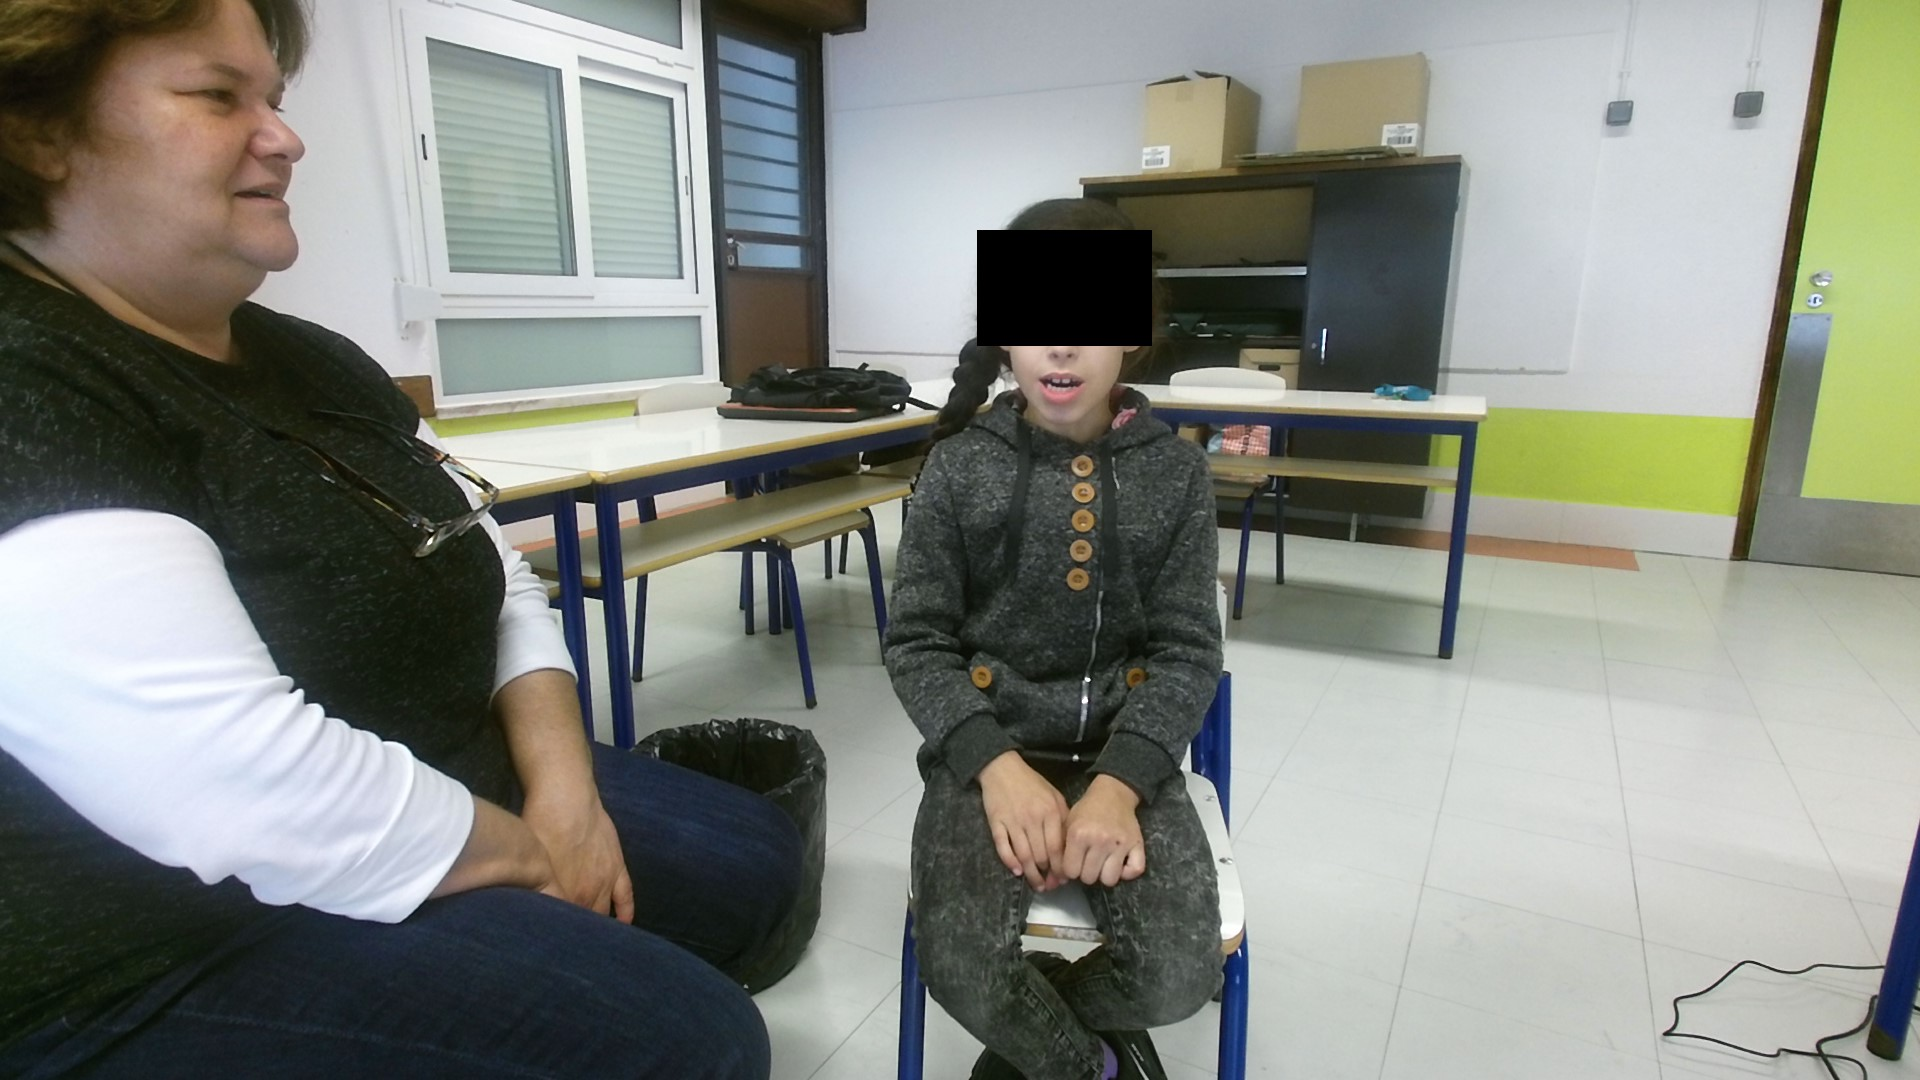
\includegraphics[trim=23cm 15cm 18cm 4cm, clip,width=0.3\linewidth]{color_639_jawFront}}    	
\subbottom[Jaw back.]{%
    \hspace{0.3cm}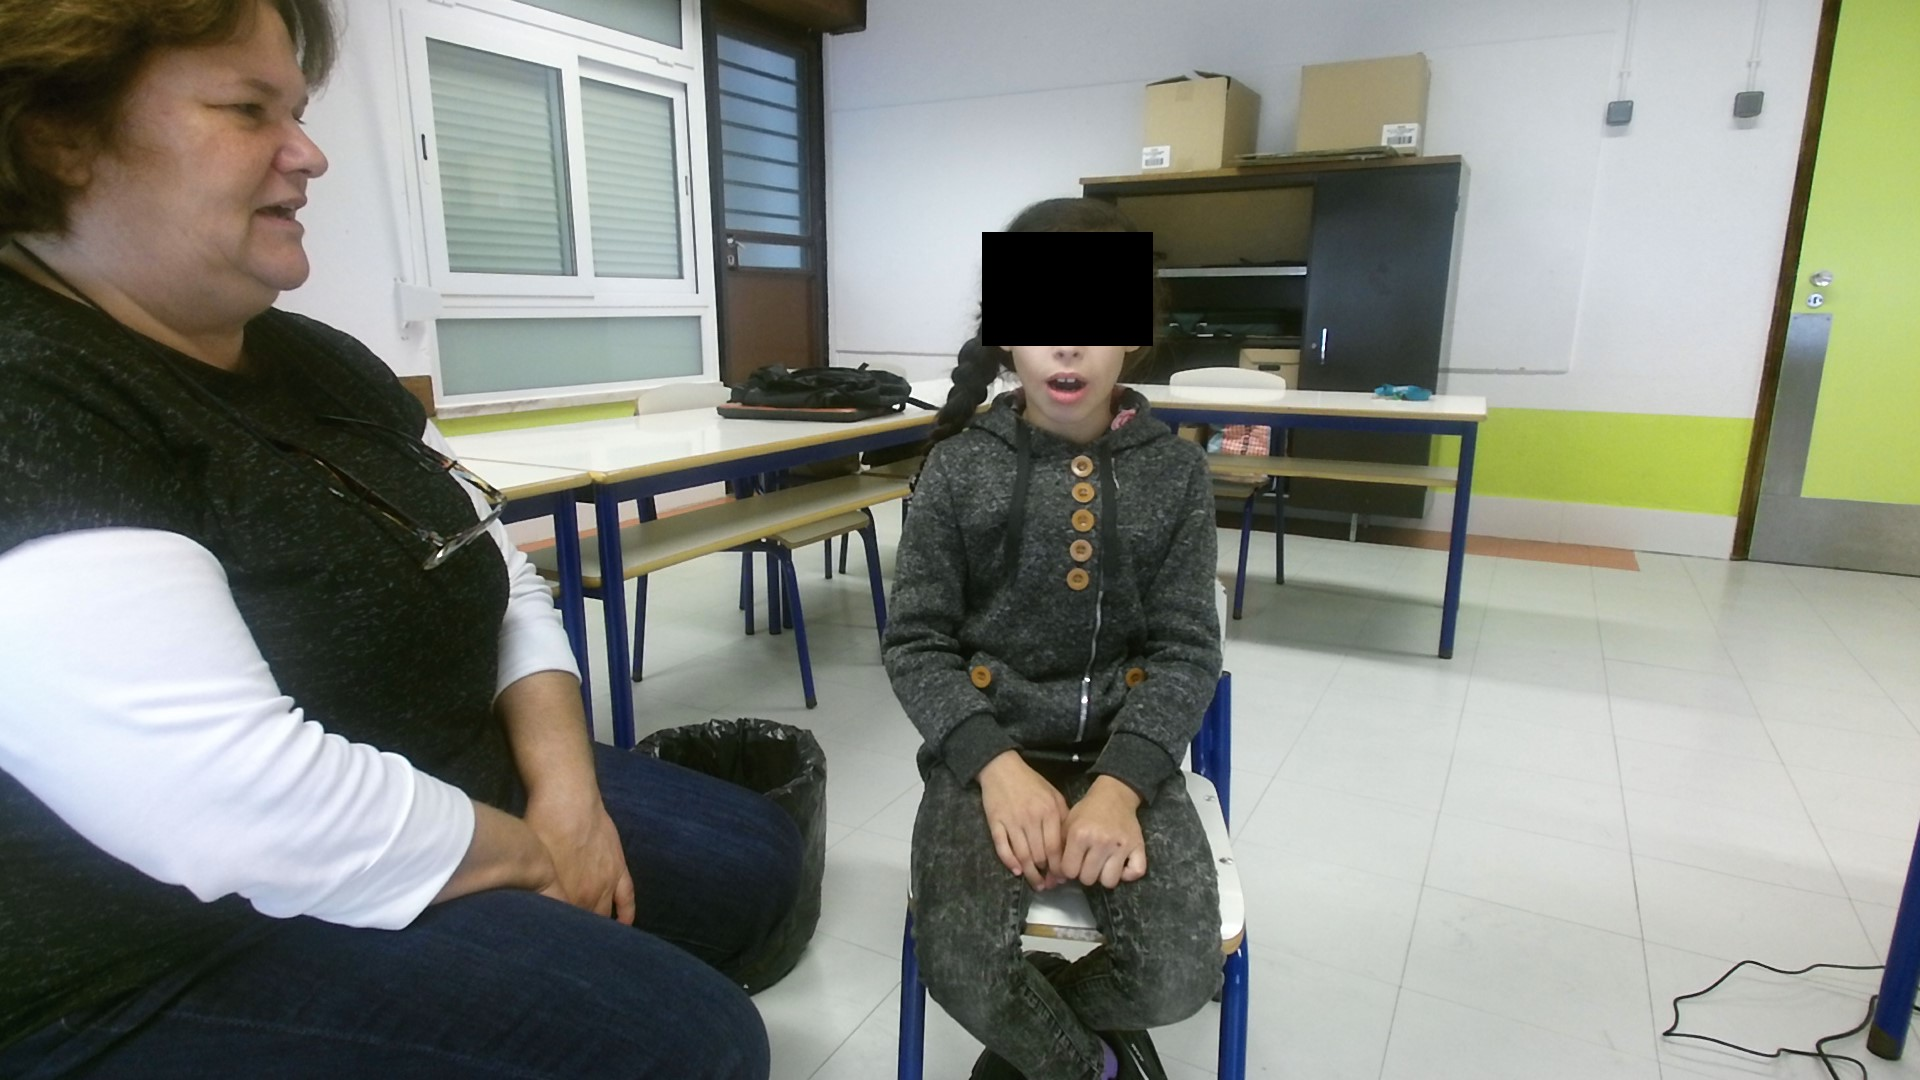
\includegraphics[trim=23cm 15cm 18cm 4cm, clip,width=0.3\linewidth]{color_642_jawBack}}%
    \subbottom[Lips over teeth.]{%
    \hspace{0.3cm}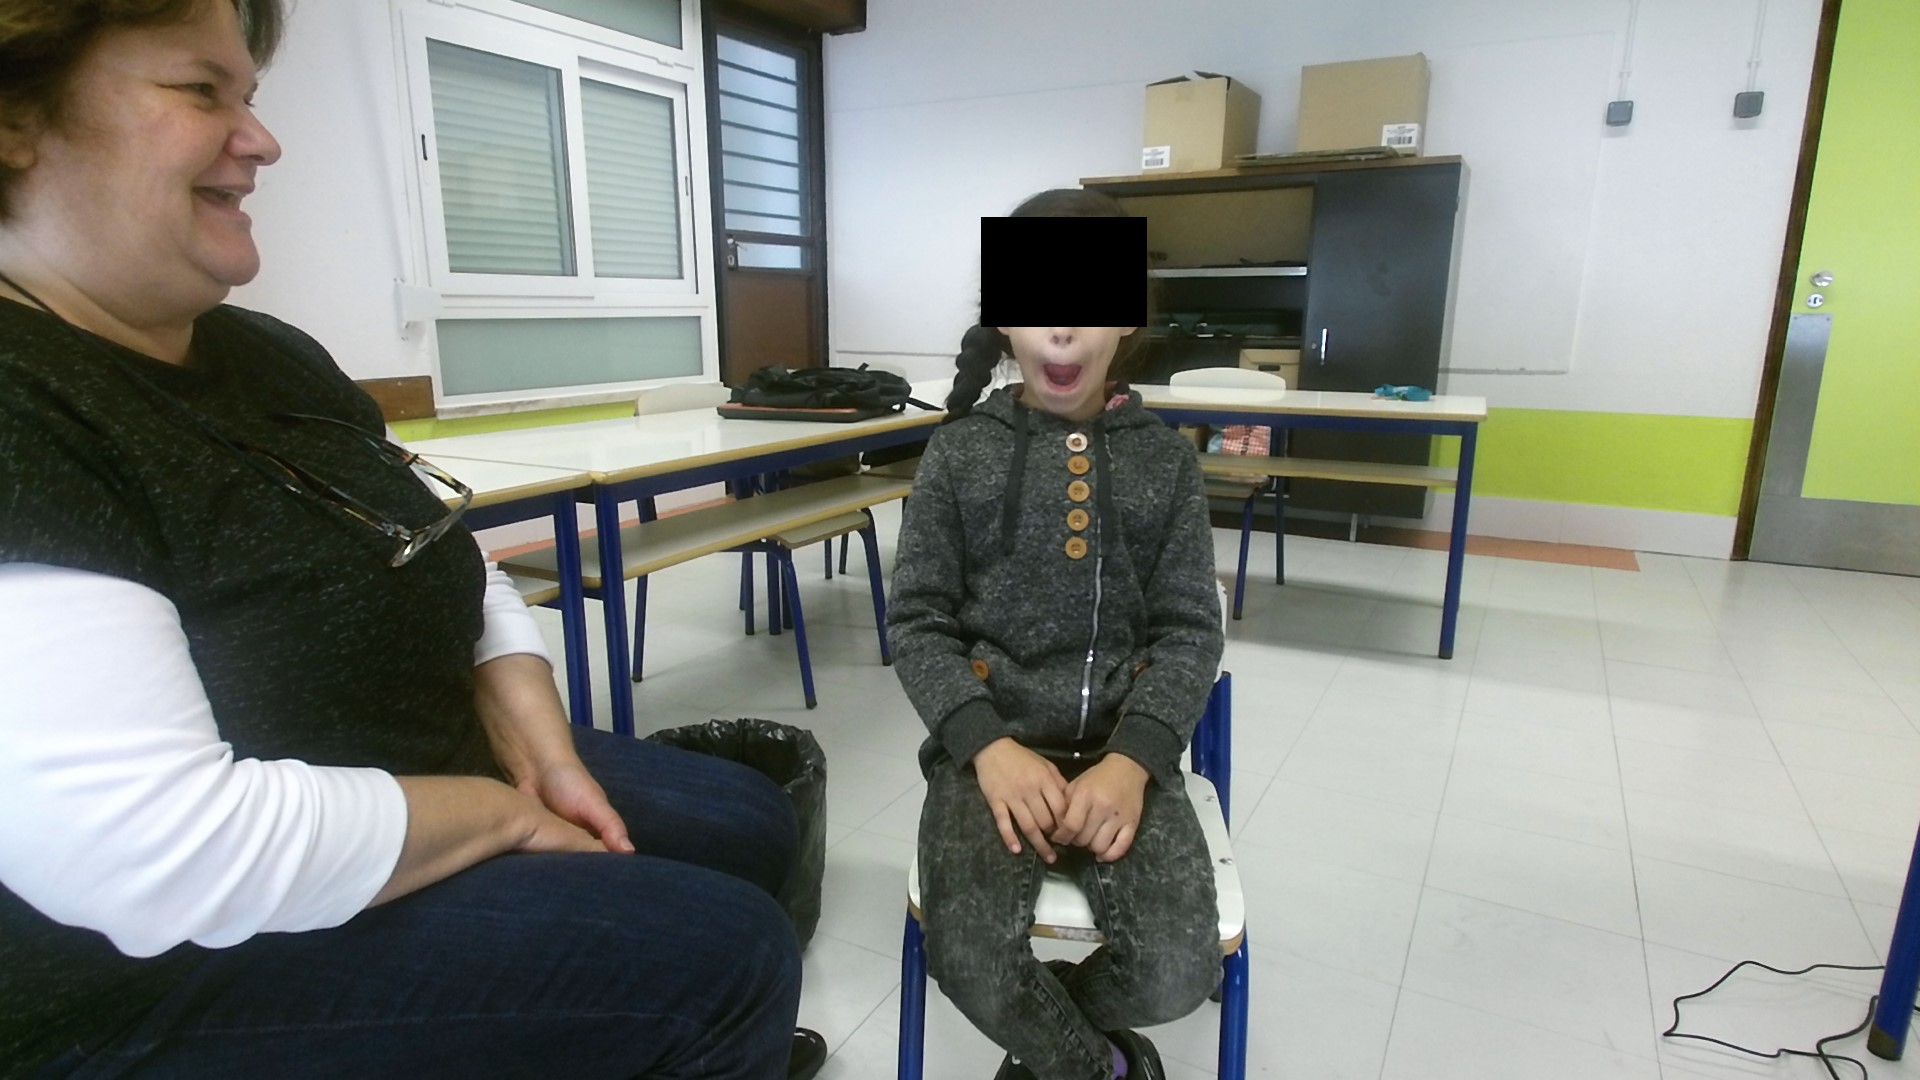
\includegraphics[trim=23cm 15cm 18cm 4cm, clip,width=0.3\linewidth]{color_202}}
\caption{Overview of performed exercises.}
\label{fig:recordedEx}
\end{figure}




\begin{figure}[htbp]
\centering
 \subbottom[]{%
    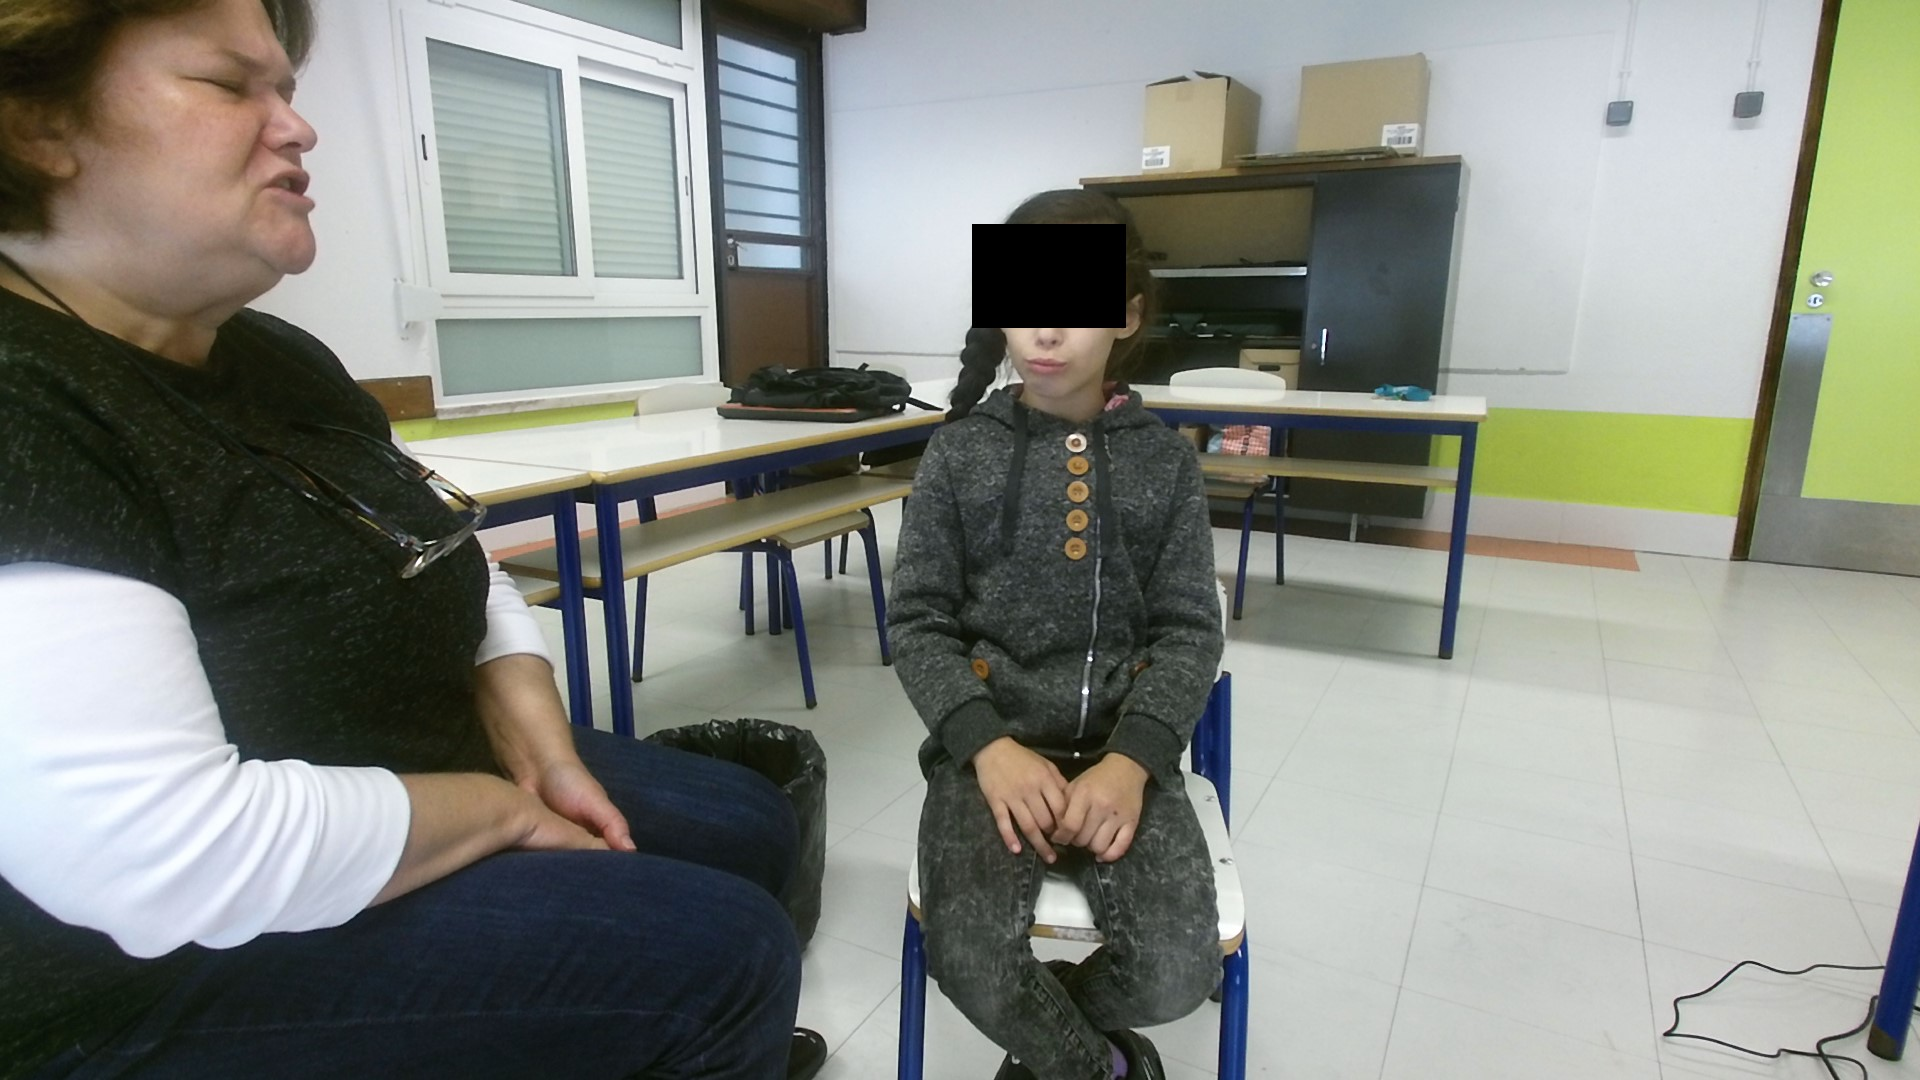
\includegraphics[trim=24cm 16cm 19cm 5cm, clip, width=0.2\linewidth]{color_193}}%
 \subbottom[]{%
    \hspace{0.3cm}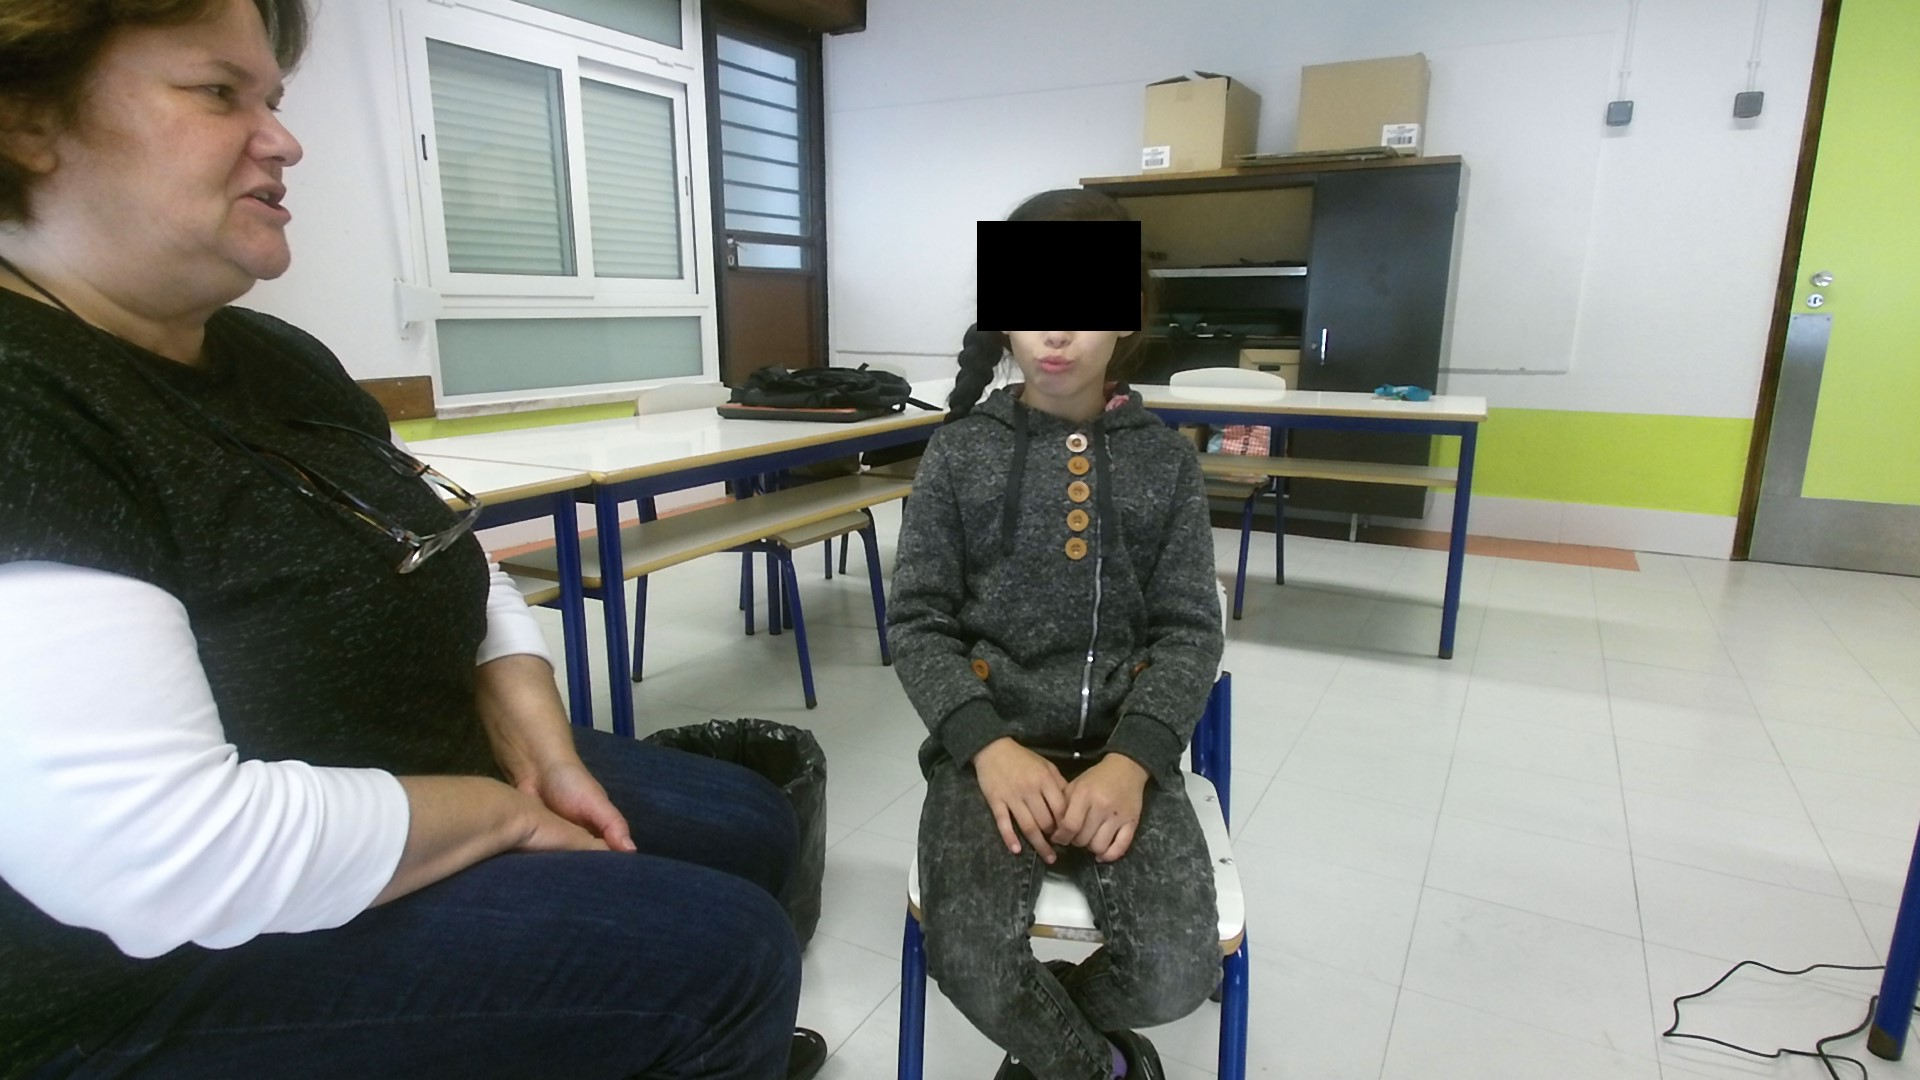
\includegraphics[trim=24cm 16cm 19cm 5cm, clip,width=0.2\linewidth]{color_194}}
 \subbottom[]{%
    \hspace{0.3cm}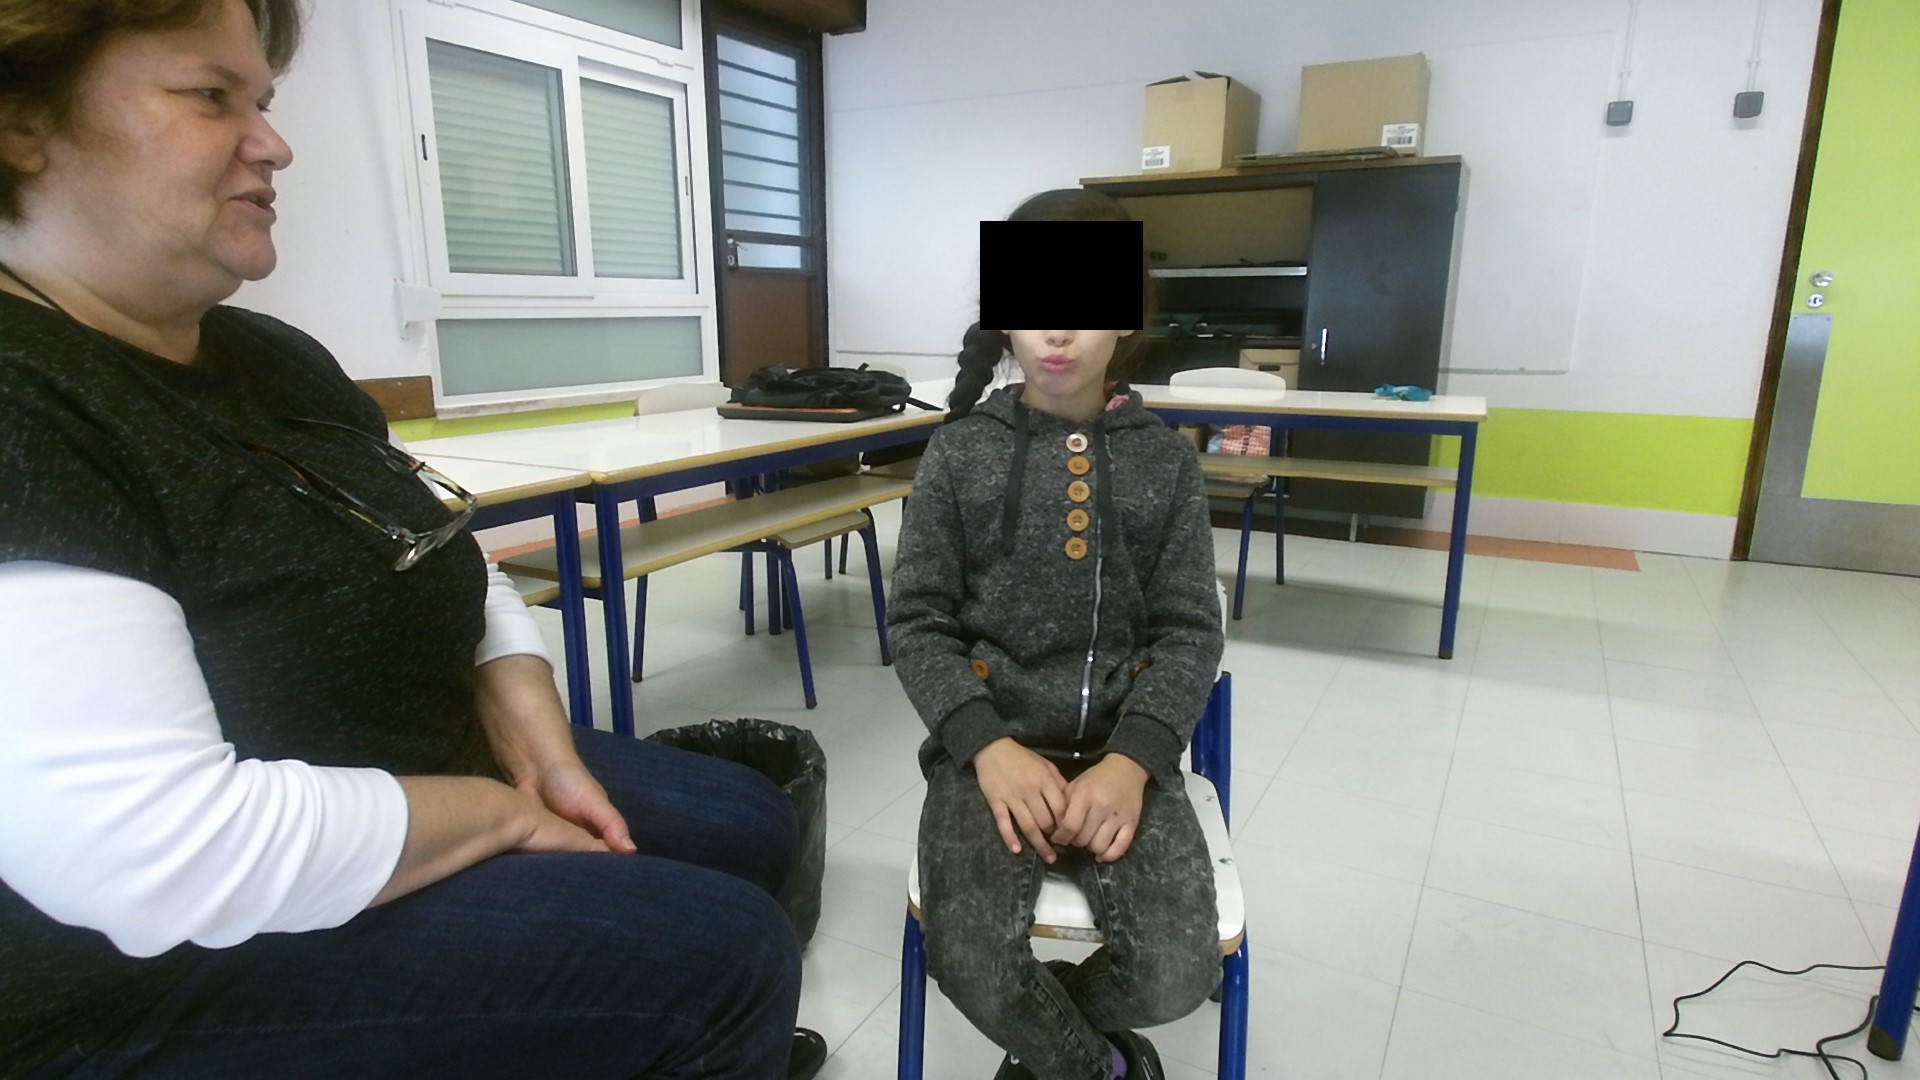
\includegraphics[trim=24cm 16cm 19cm 5cm, clip,width=0.2\linewidth]{color_195}}
    \subbottom[]{%
    \hspace{0.3cm}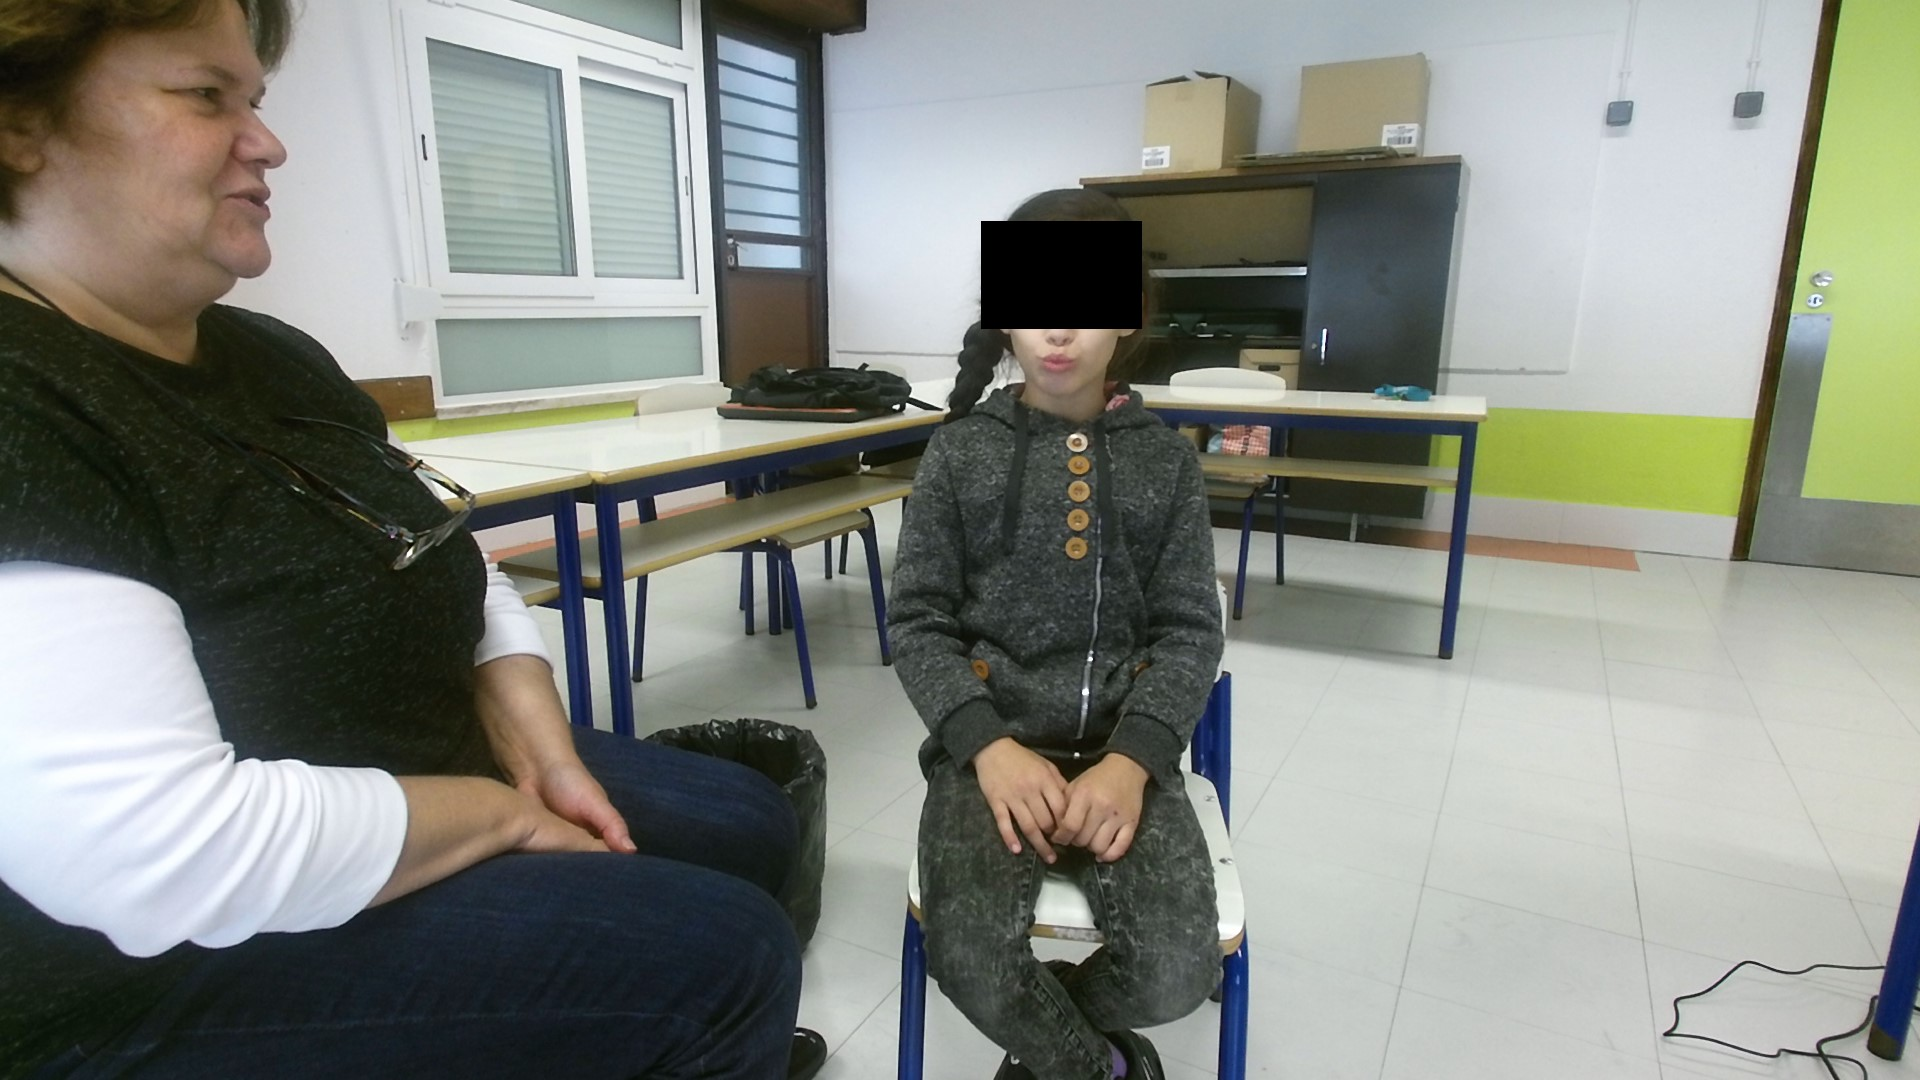
\includegraphics[trim=24cm 16cm 19cm 5cm, clip,width=0.2\linewidth]{color_196}}\\ 
 \subbottom[]{%
    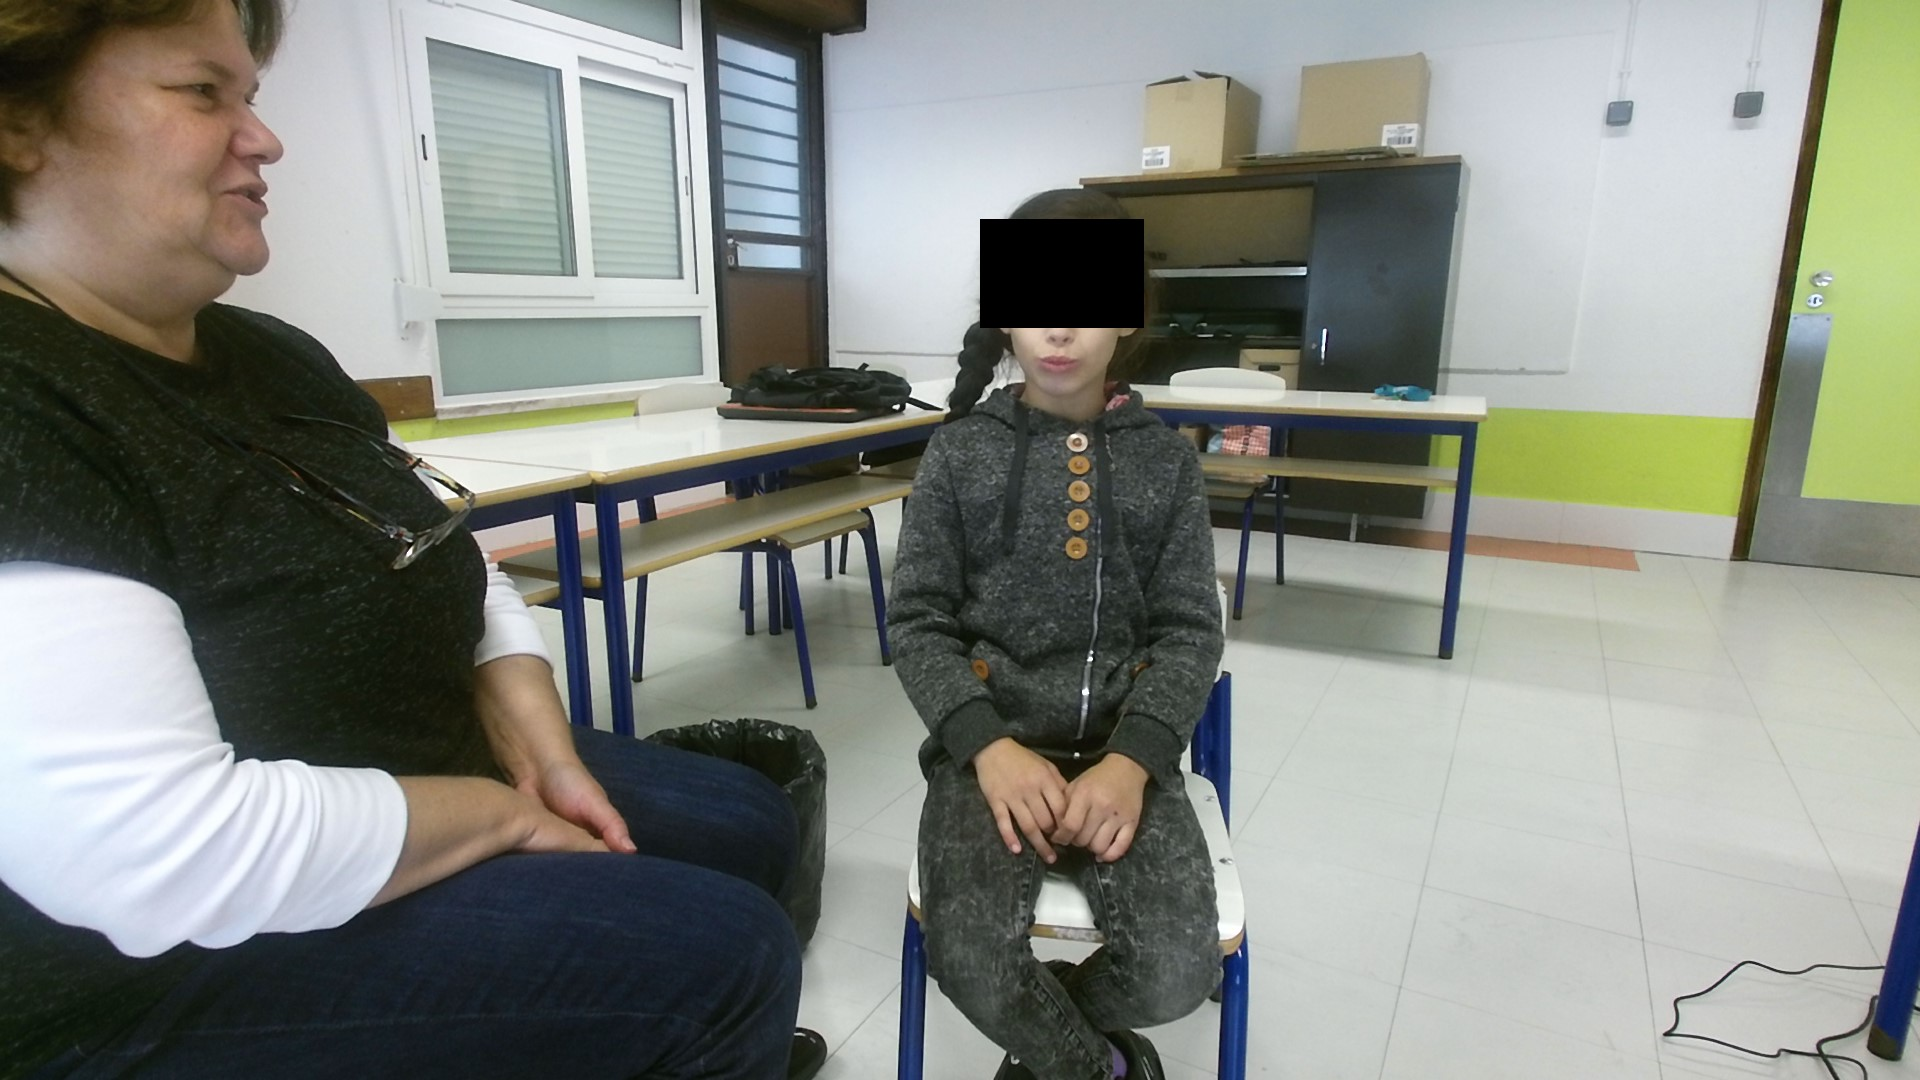
\includegraphics[trim=24cm 16cm 19cm 5cm, clip,width=0.2\linewidth]{color_197}}    	
\subbottom[]{%
    \hspace{0.3cm}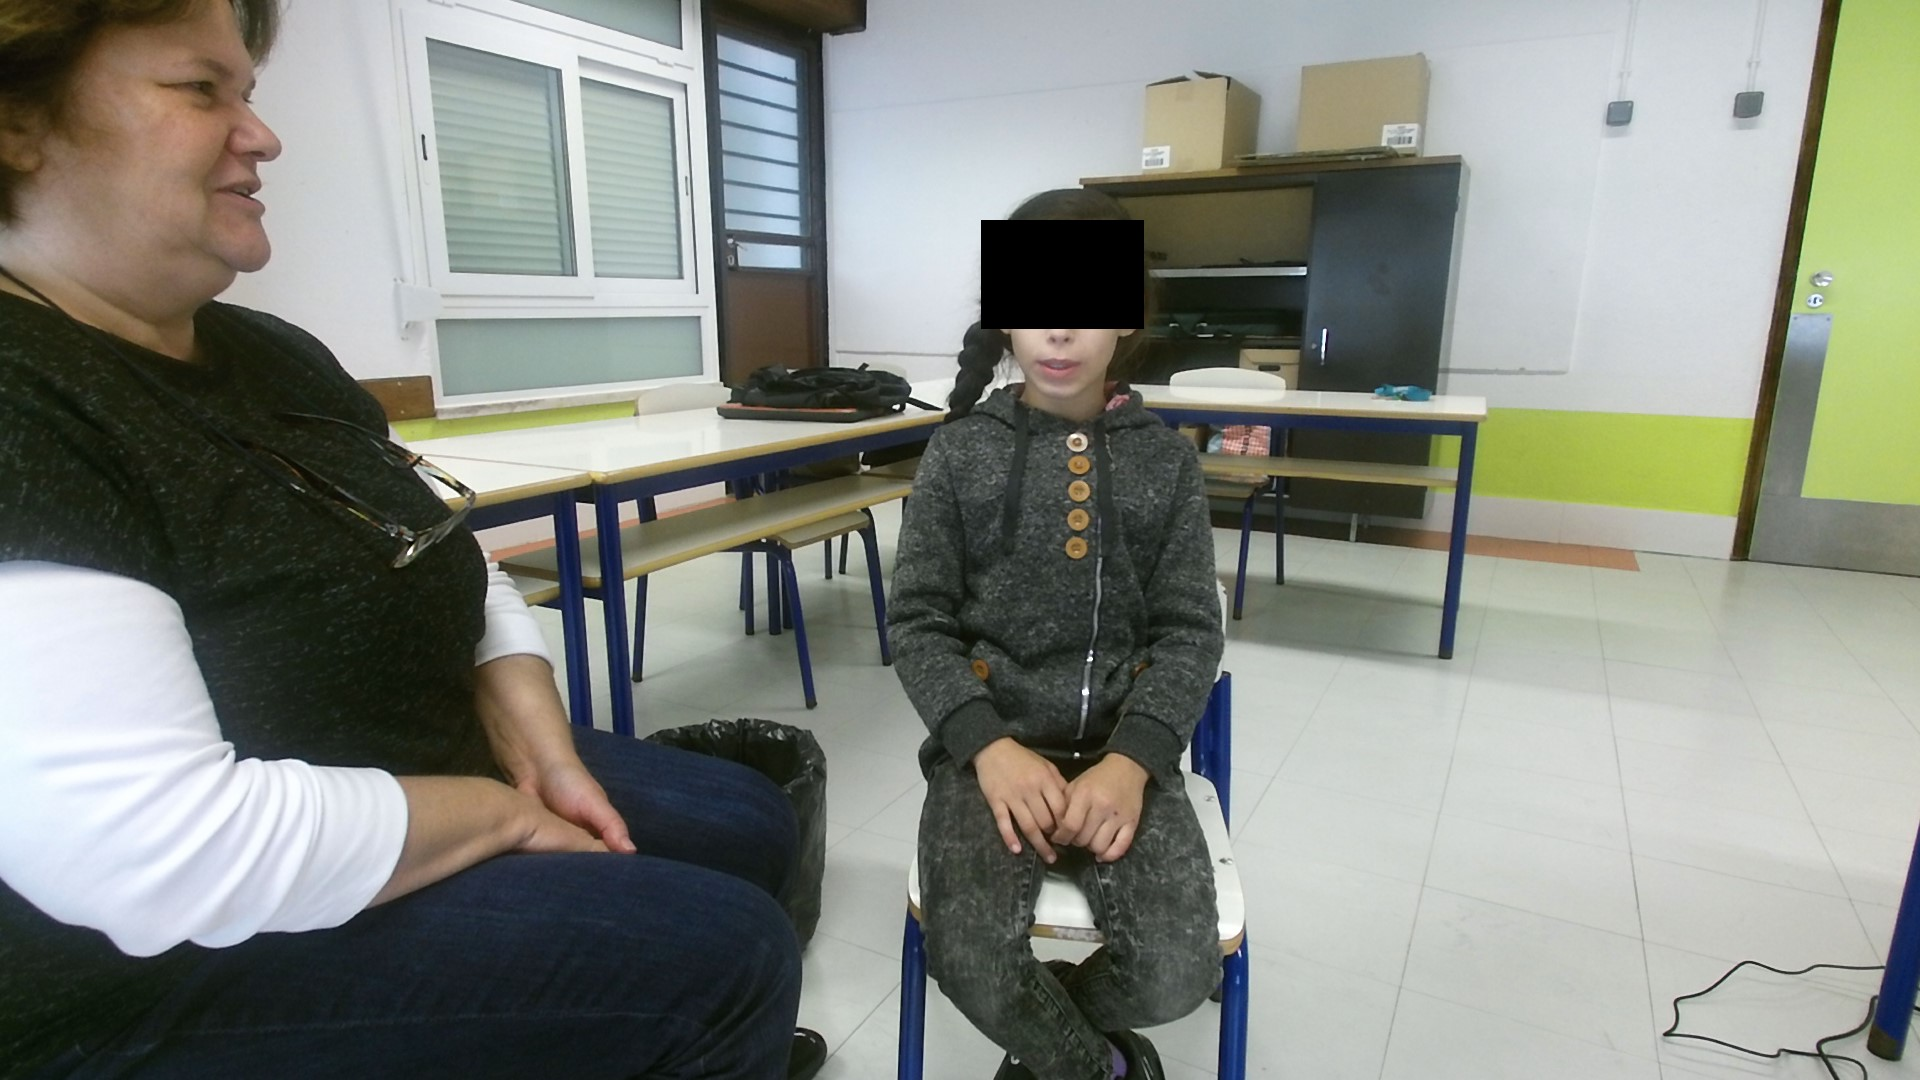
\includegraphics[trim=24cm 16cm 19cm 5cm, clip,width=0.2\linewidth]{color_198}}
 \subbottom[]{%
    \hspace{0.3cm}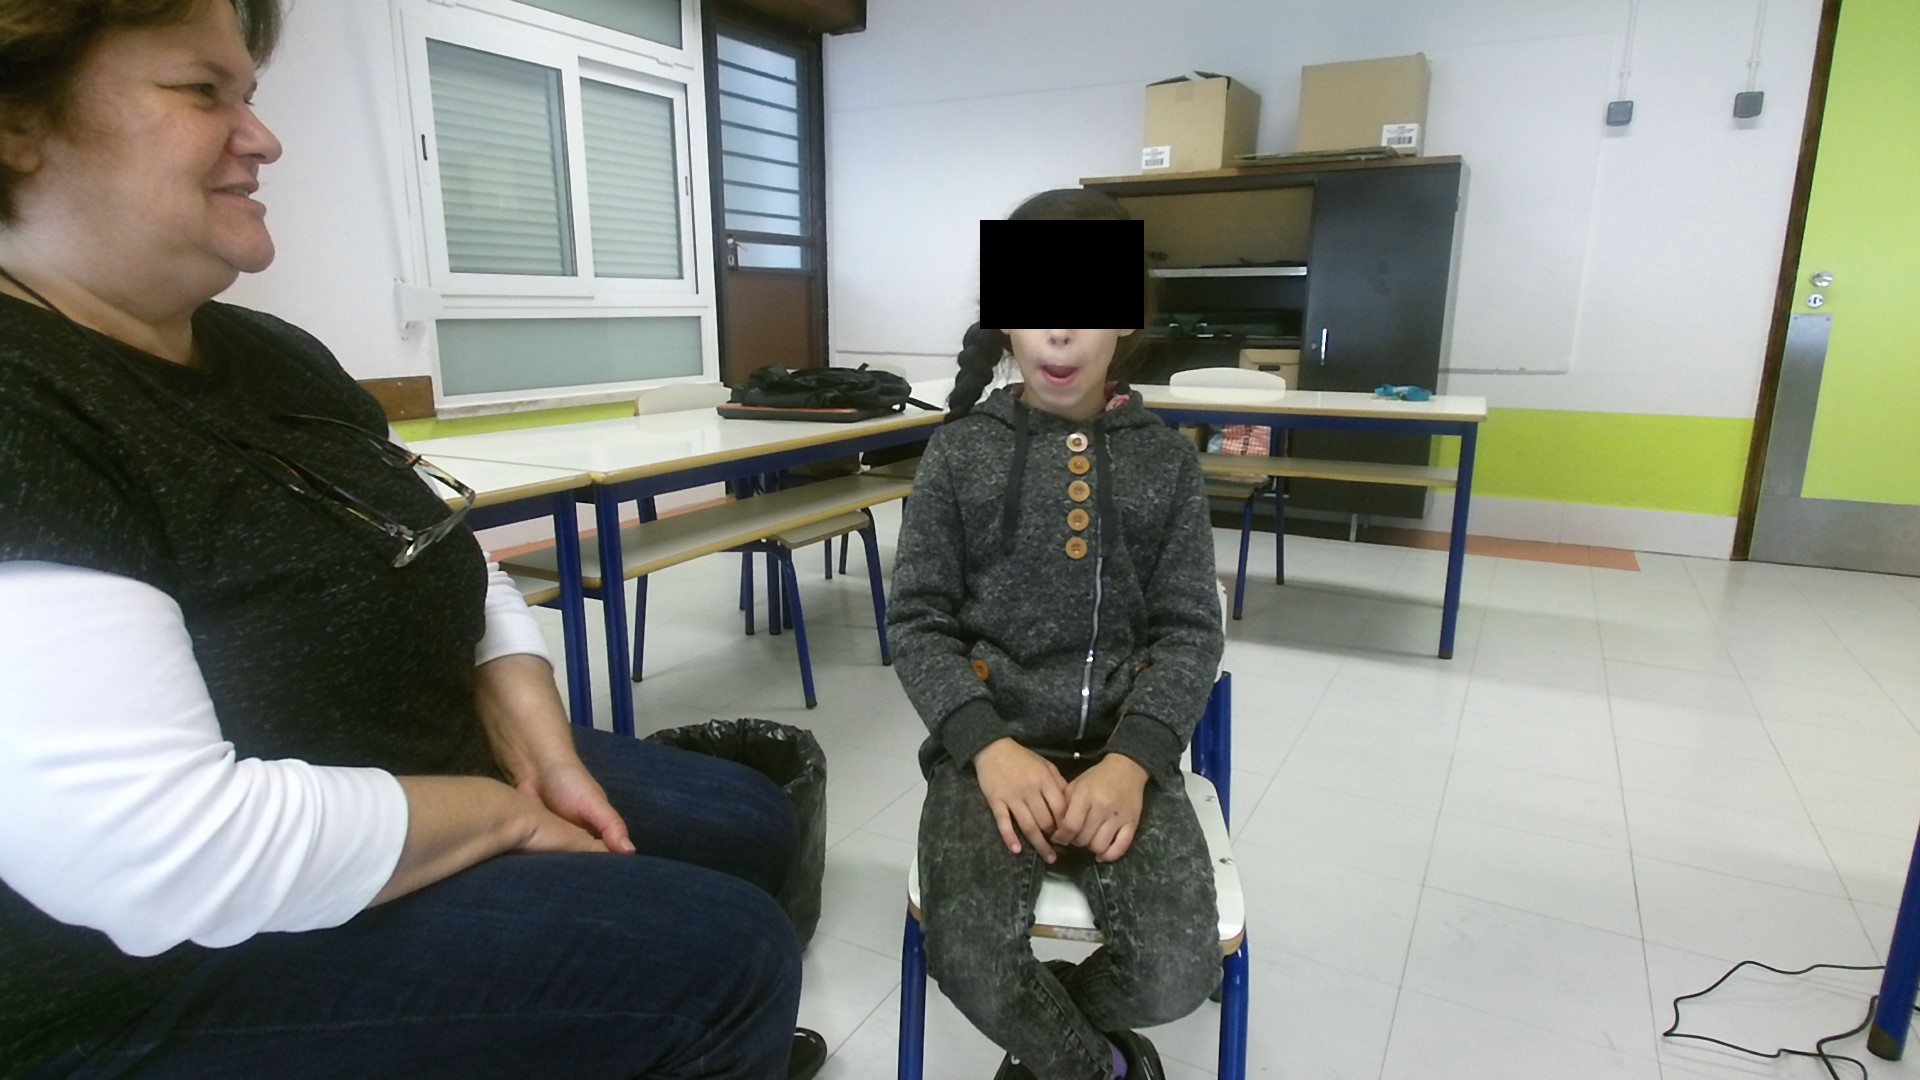
\includegraphics[trim=24cm 16cm 19cm 5cm, clip,width=0.2\linewidth]{color_199}}    	
\subbottom[]{%
    \hspace{0.3cm}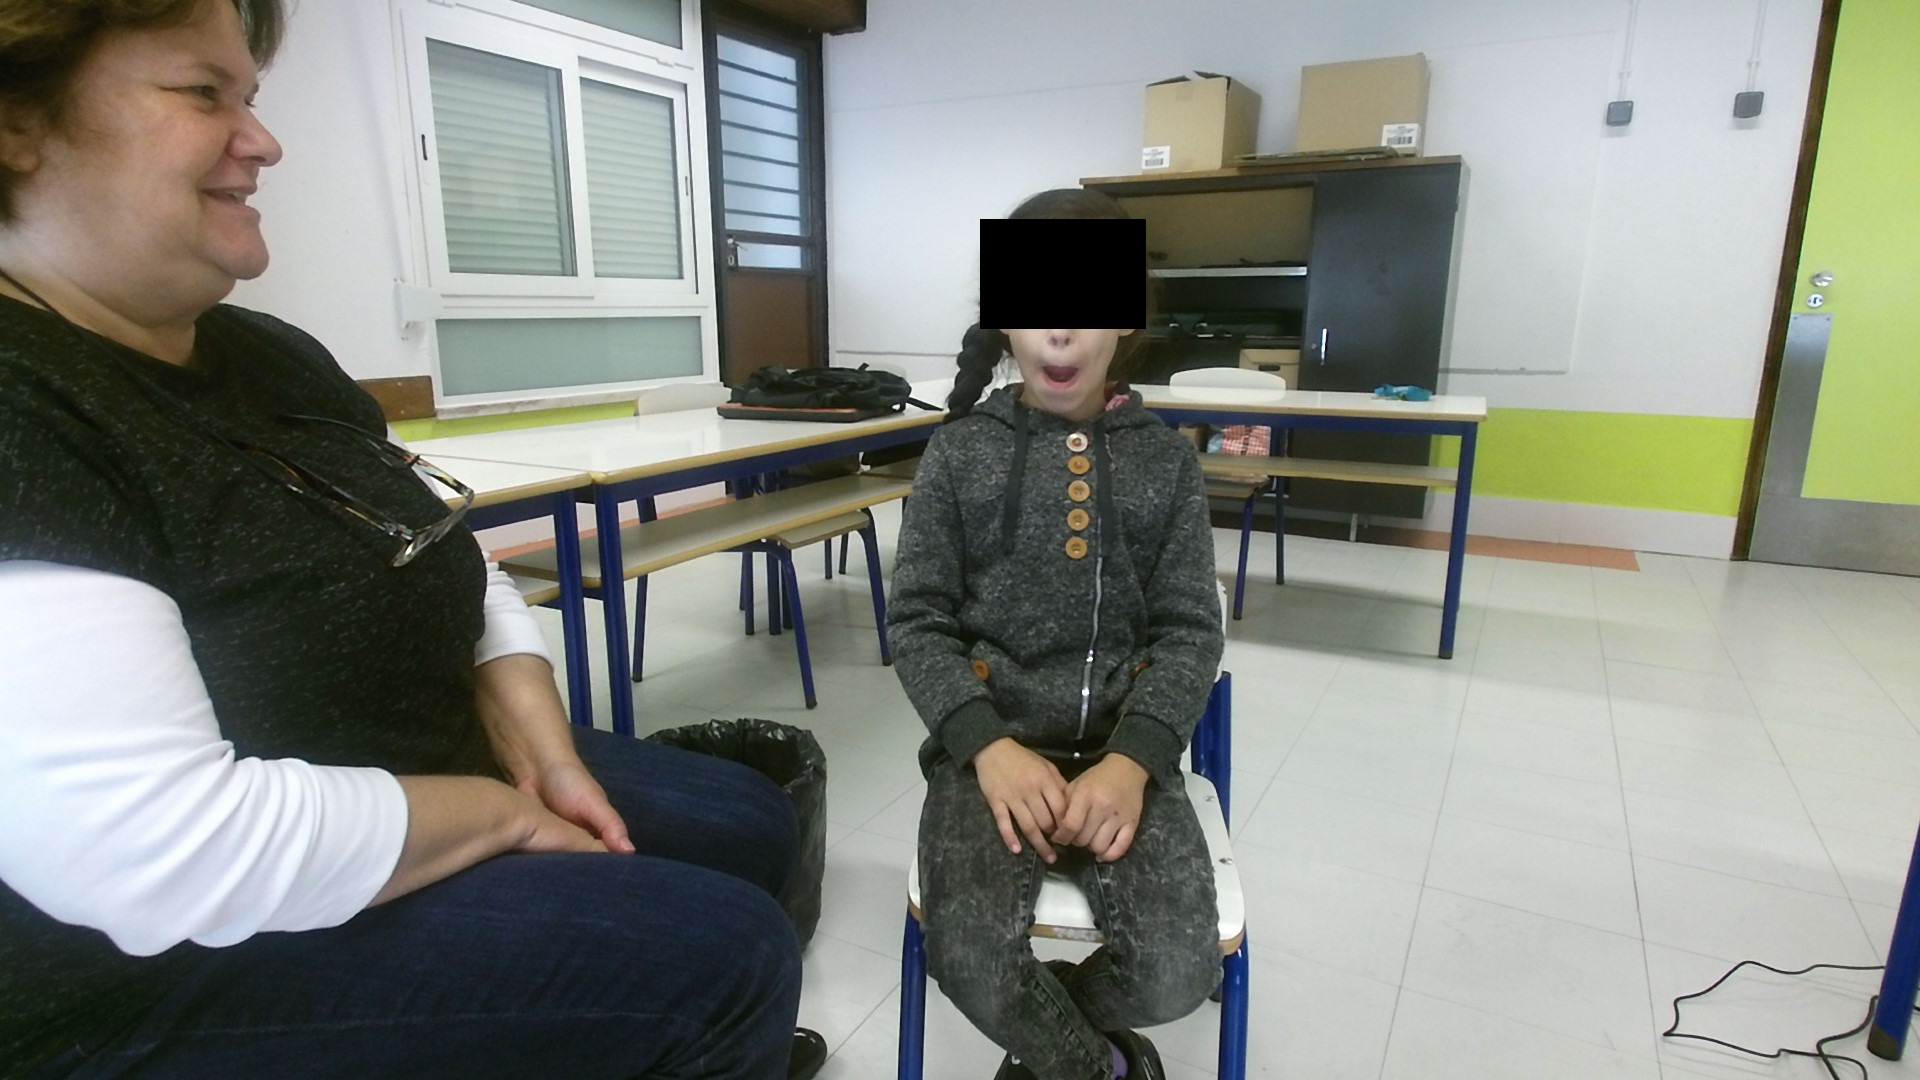
\includegraphics[trim=24cm 16cm 19cm 5cm, clip,width=0.2\linewidth]{color_200}}\\
\subbottom[]{%
    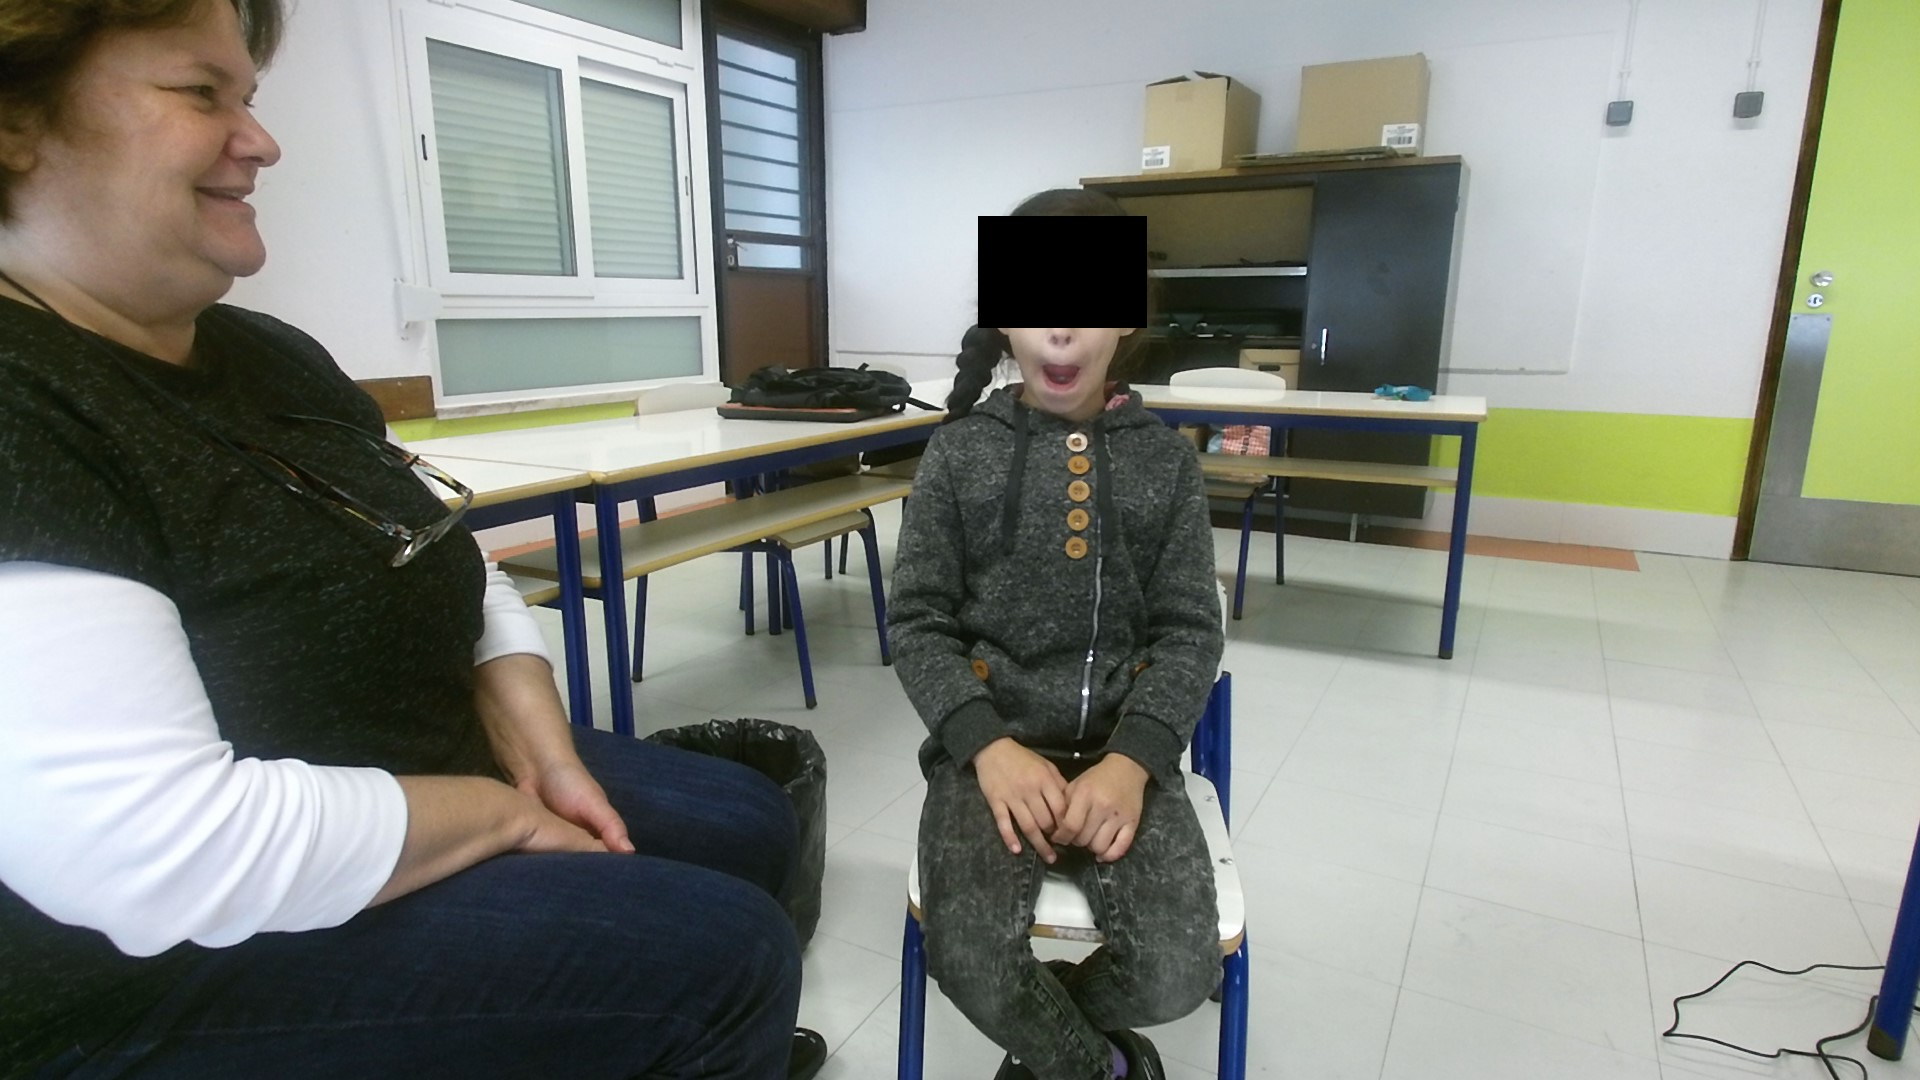
\includegraphics[trim=24cm 16cm 19cm 5cm, clip,width=0.2\linewidth]{color_201}}
\subbottom[]{%
    \hspace{0.3cm}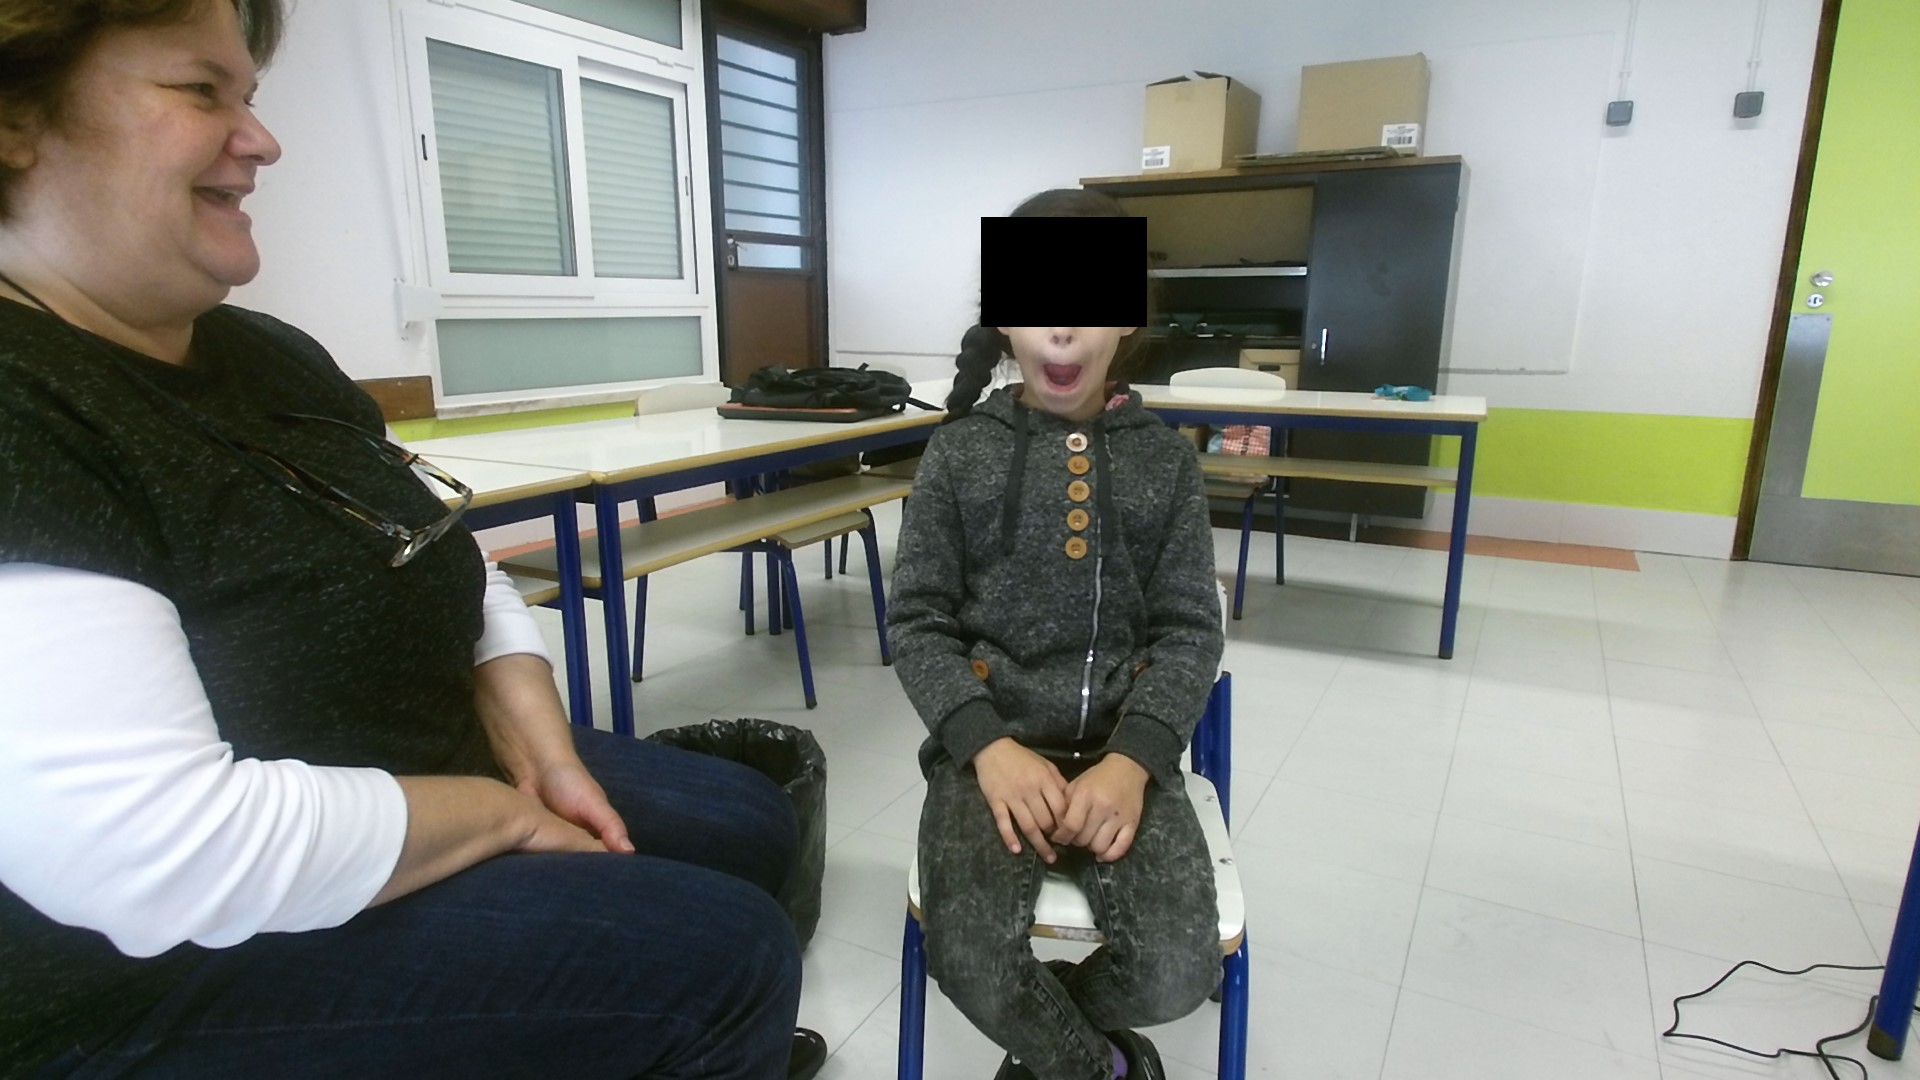
\includegraphics[trim=24cm 16cm 19cm 5cm, clip,width=0.2\linewidth]{color_202}}
\subbottom[]{%
    \hspace{0.3cm}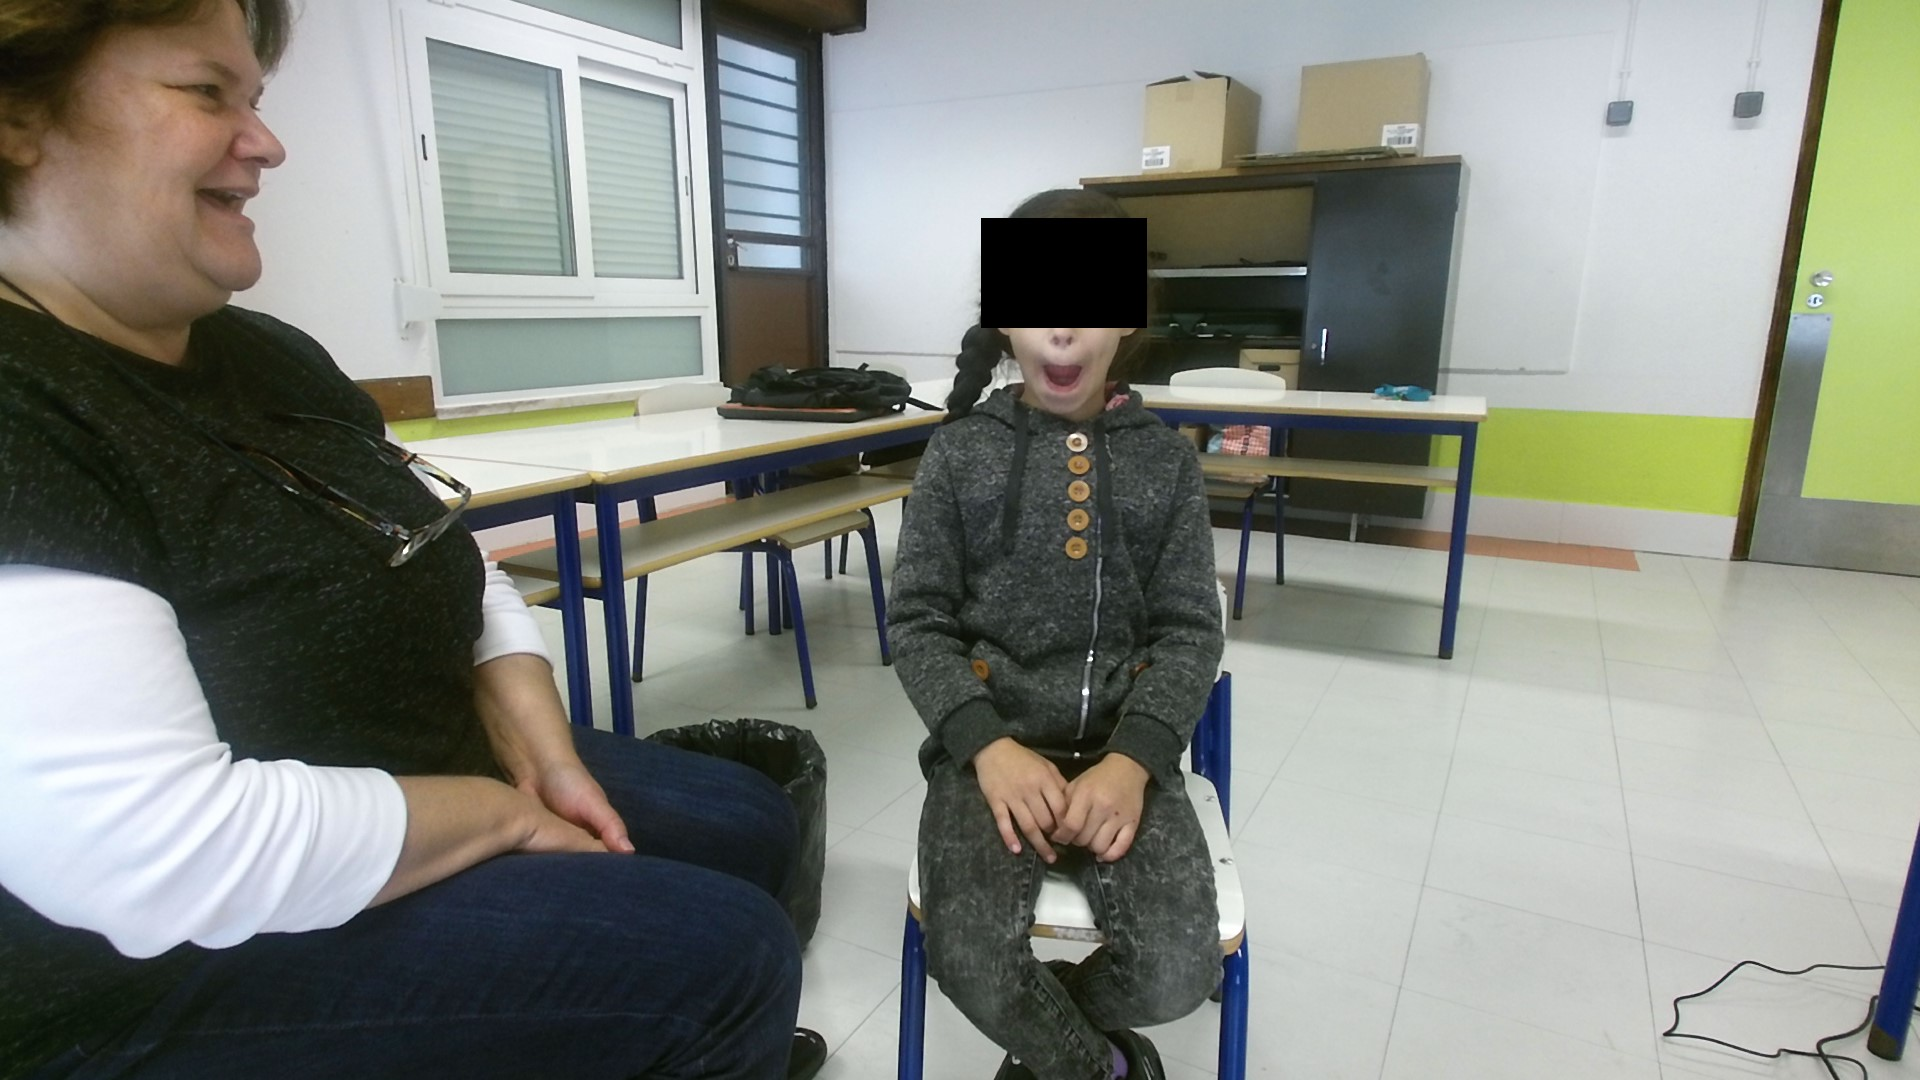
\includegraphics[trim=24cm 16cm 19cm 5cm, clip,width=0.2\linewidth]{color_203}}
\subbottom[]{%
    \hspace{0.3cm}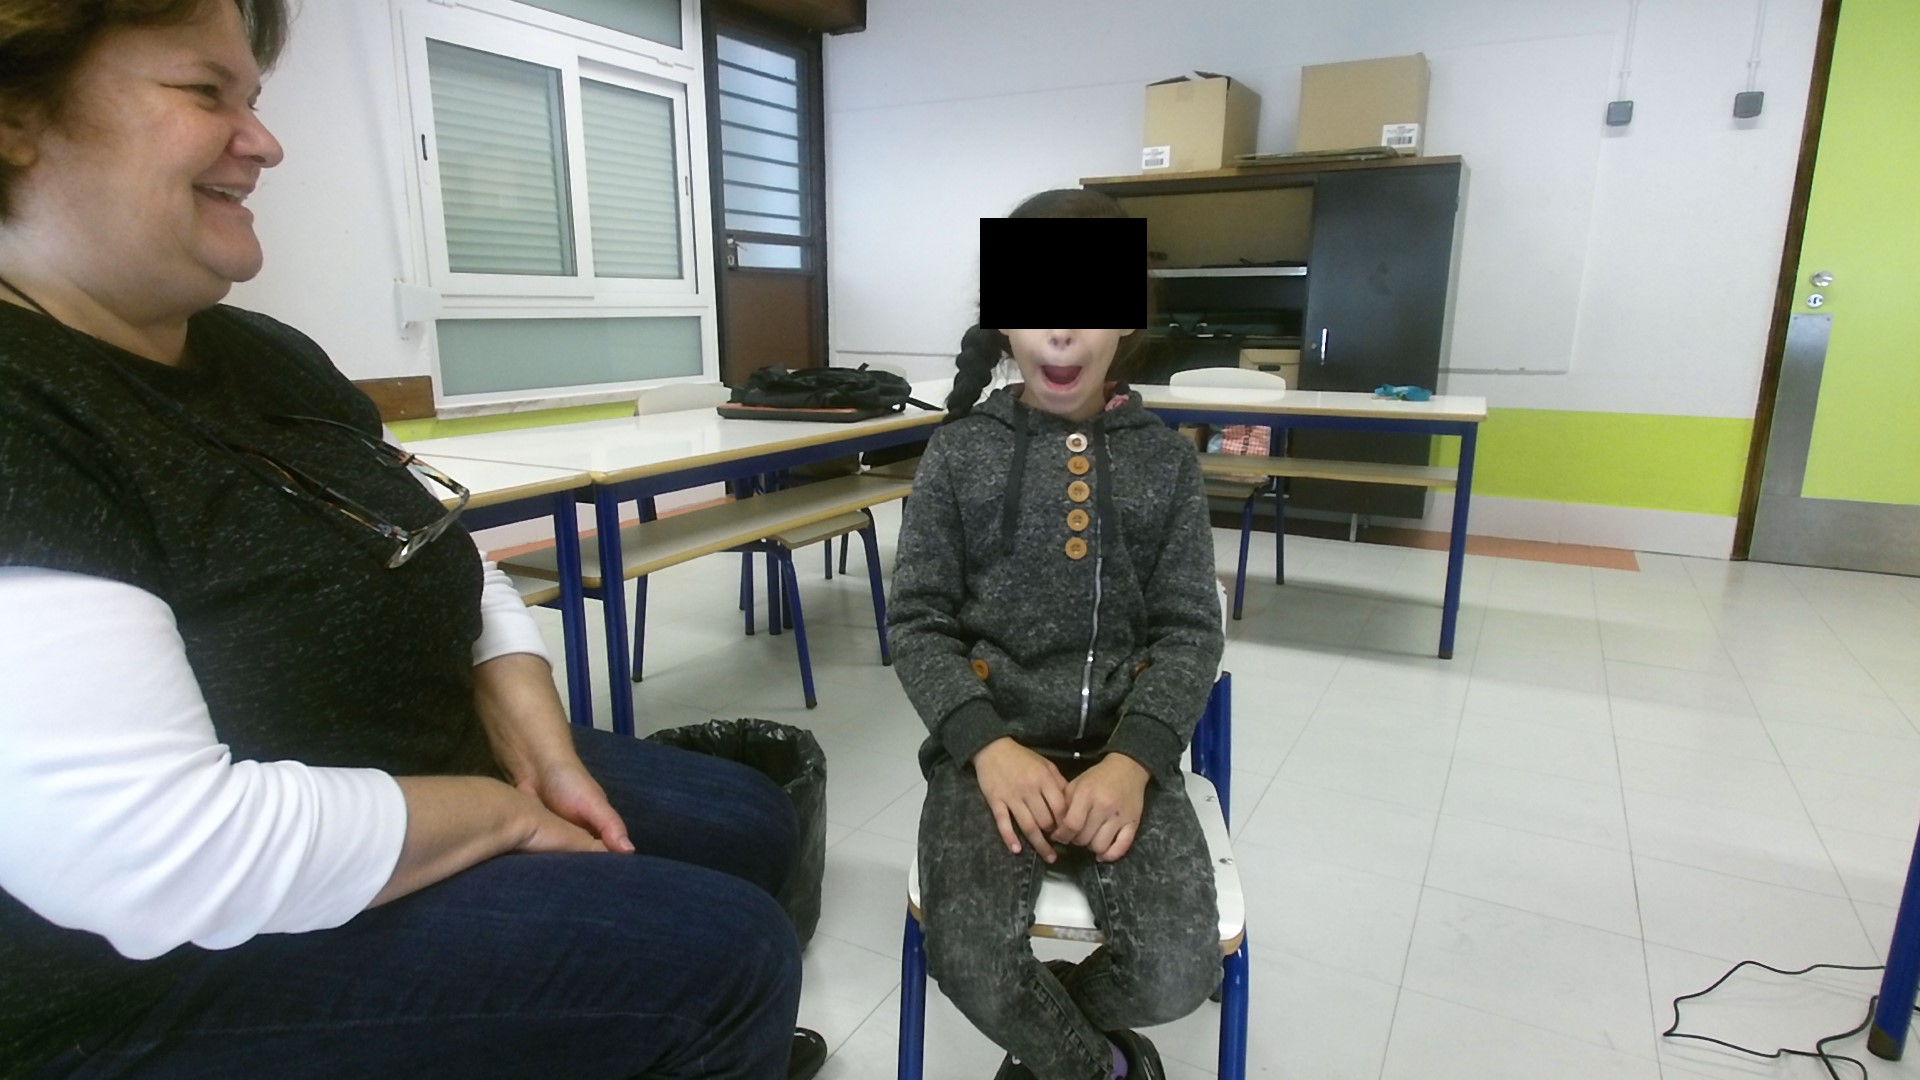
\includegraphics[trim=24cm 16cm 19cm 5cm, clip,width=0.2\linewidth]{color_204}}\\
    \subbottom[]{%
    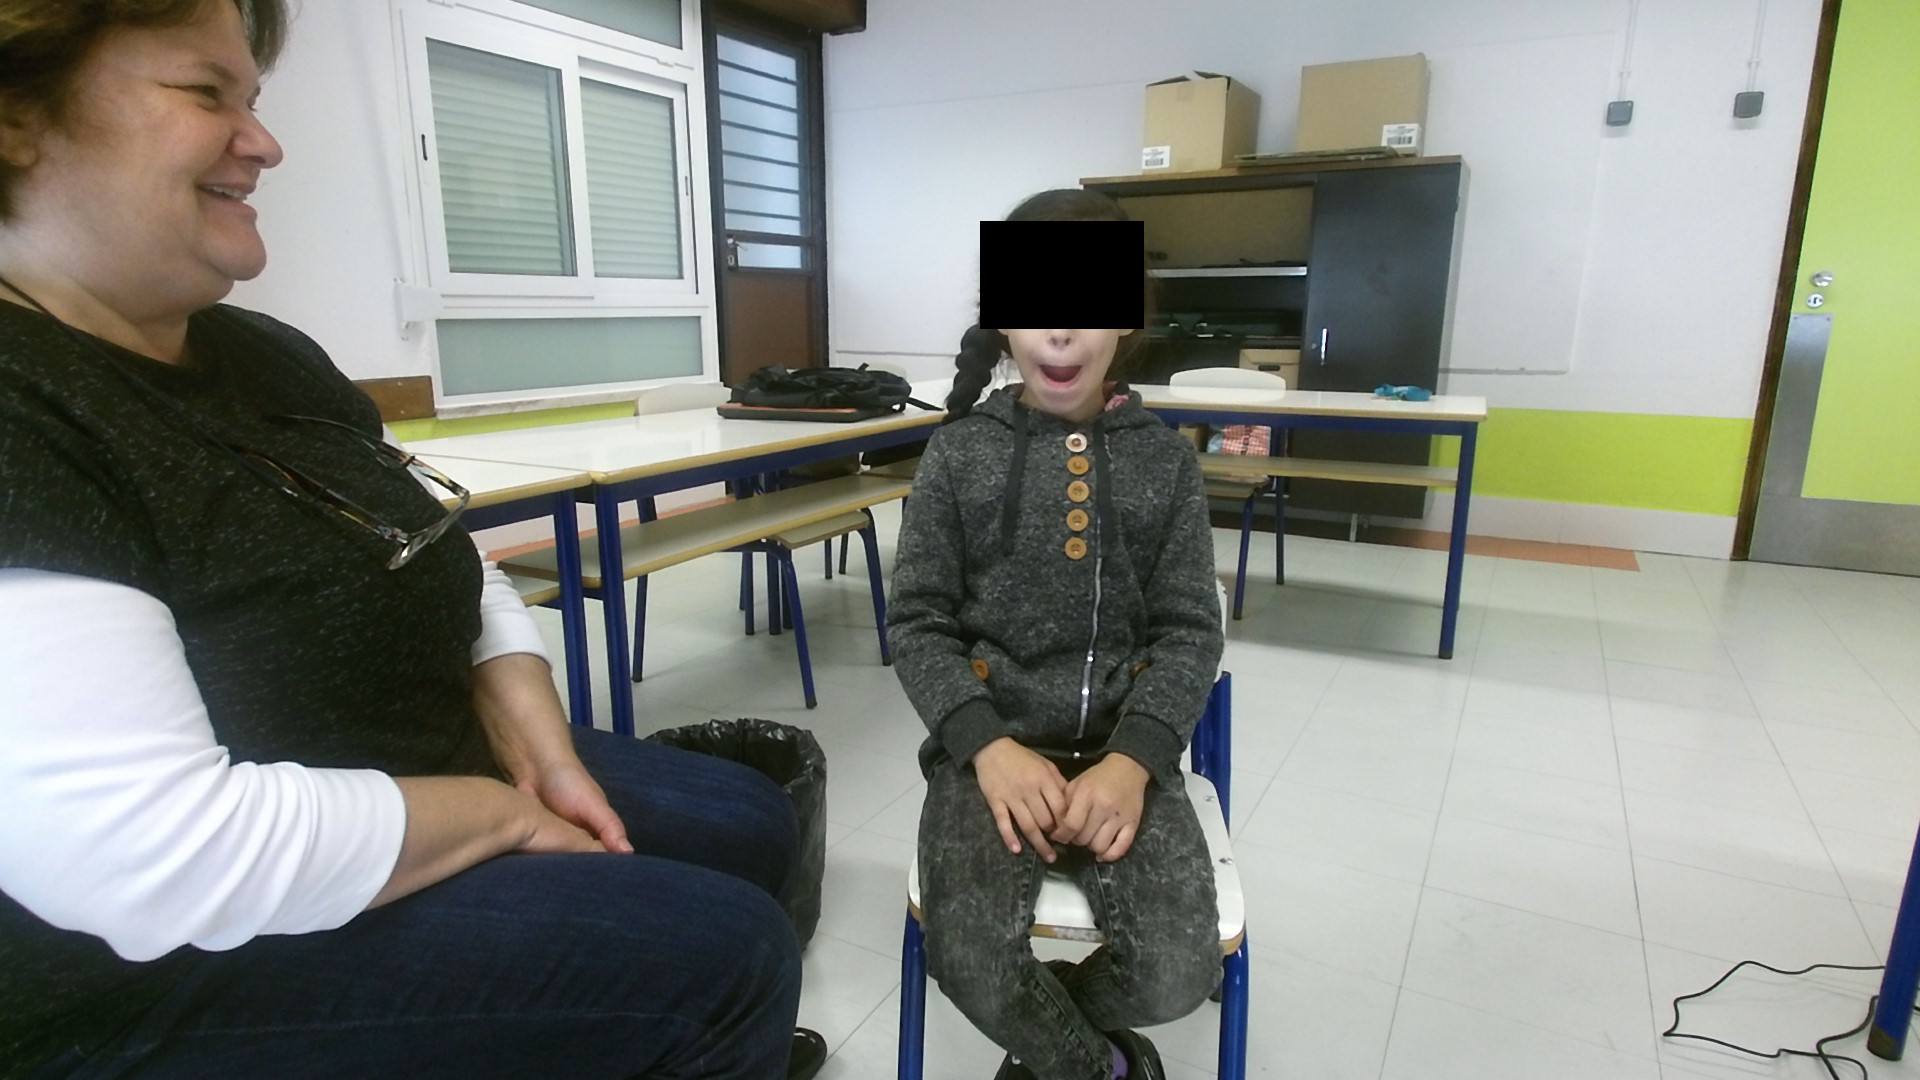
\includegraphics[trim=24cm 16cm 19cm 5cm, clip,width=0.2\linewidth]{color_205}}
\subbottom[]{%
    \hspace{0.3cm}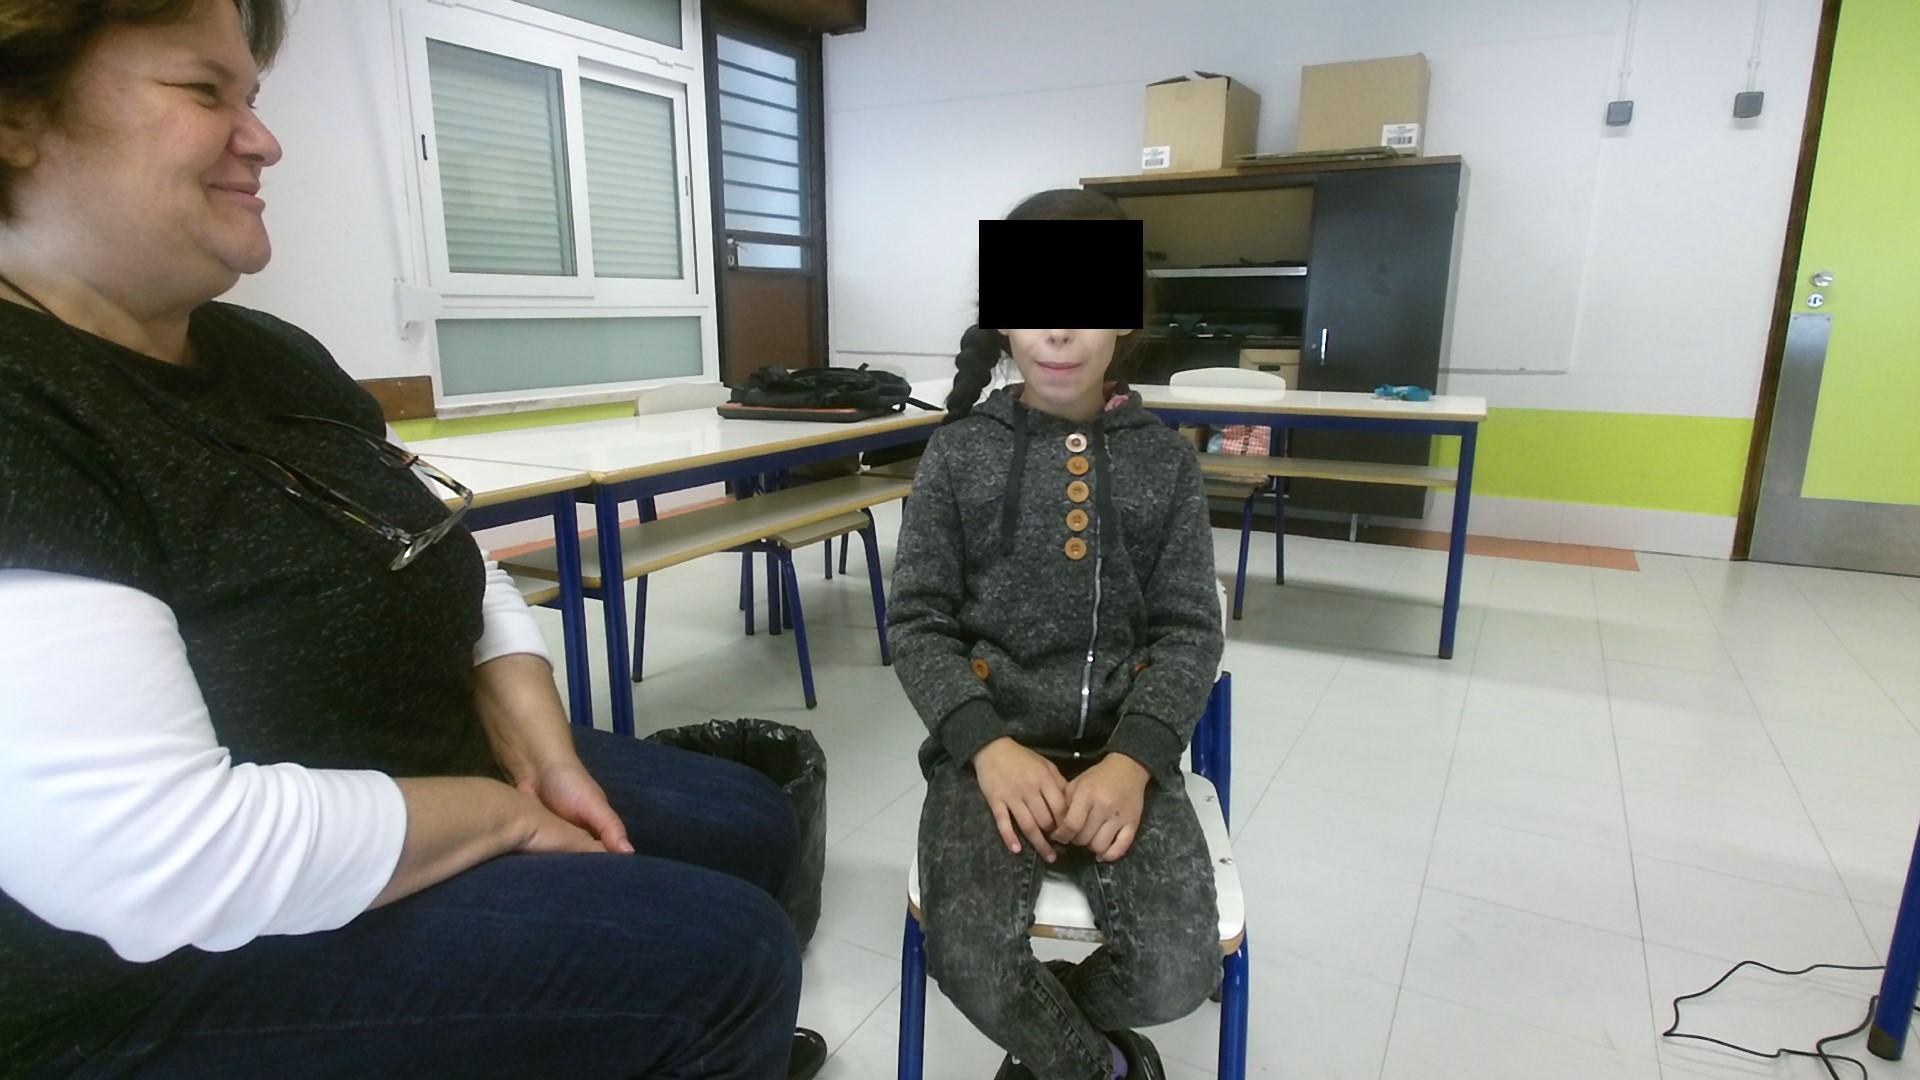
\includegraphics[trim=24cm 16cm 19cm 5cm, clip,width=0.2\linewidth]{color_206}}
\subbottom[]{%
    \hspace{0.3cm}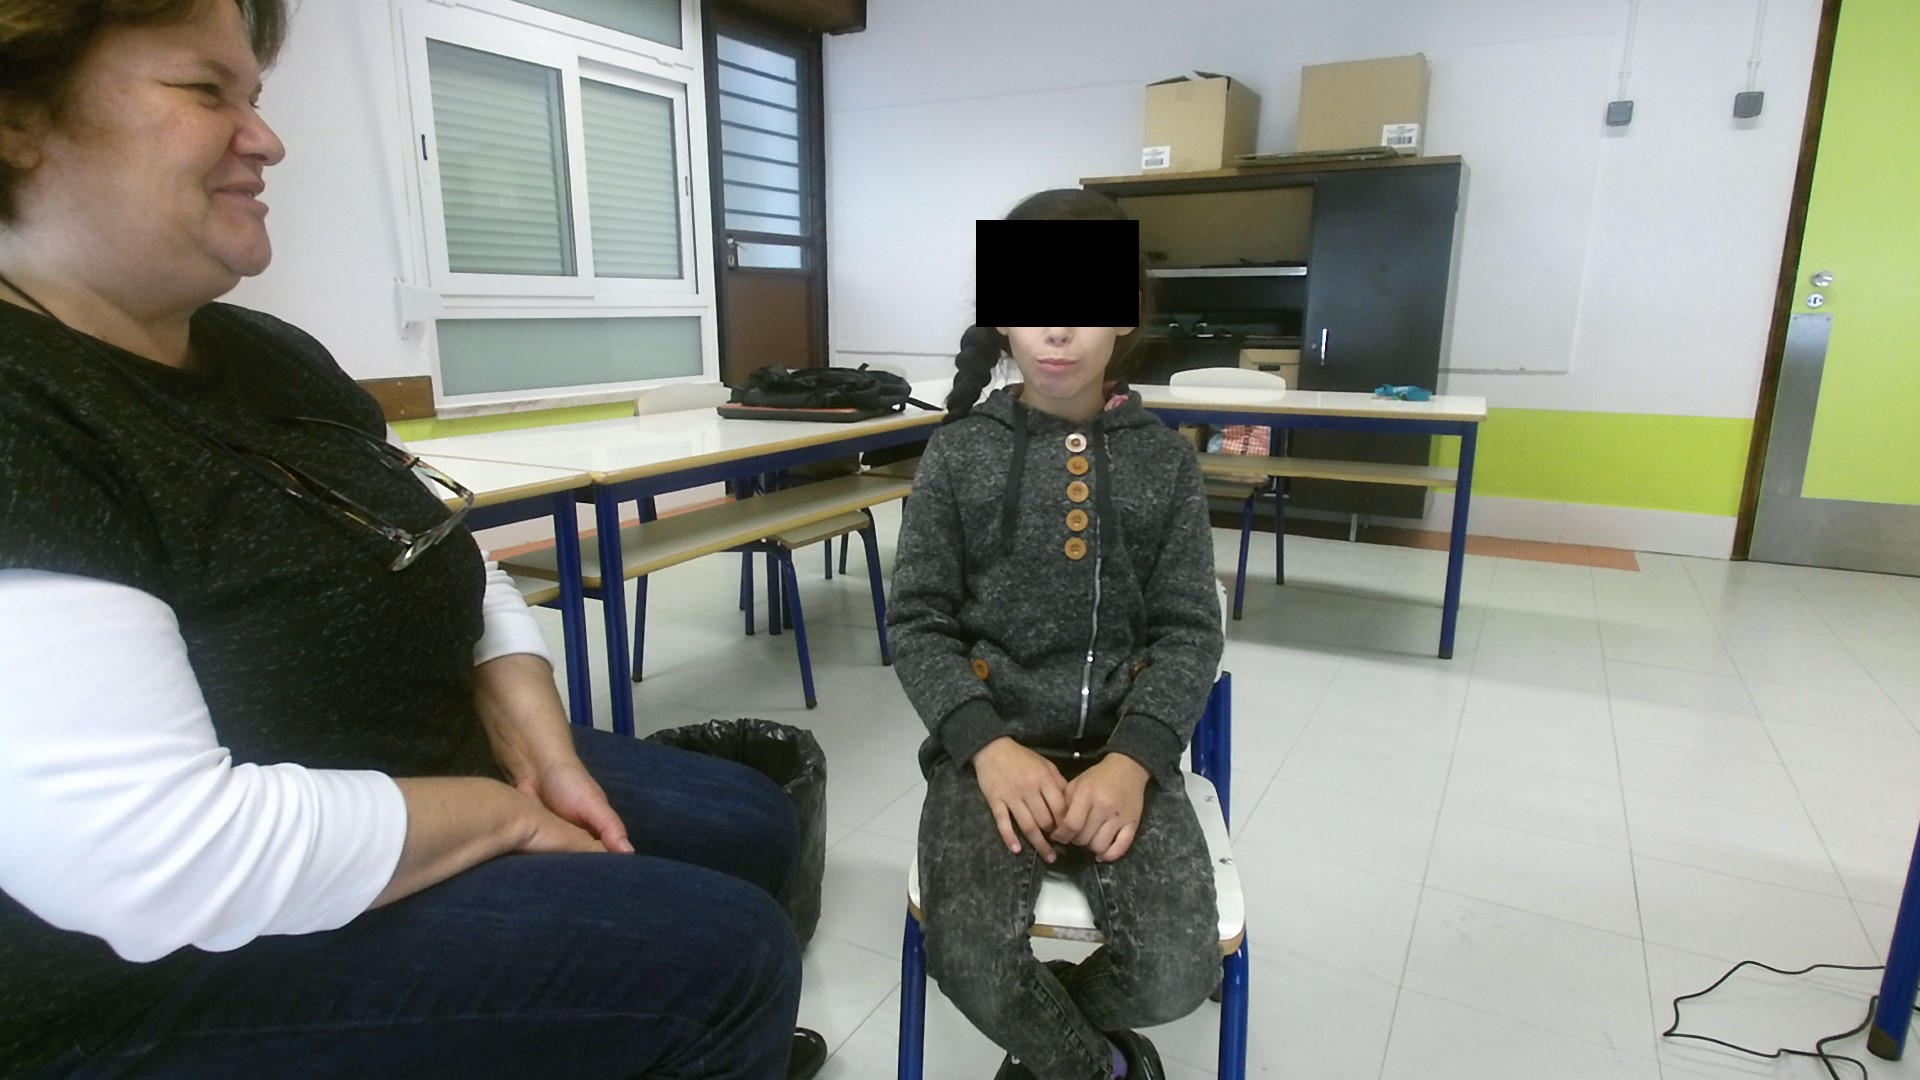
\includegraphics[trim=24cm 16cm 19cm 5cm, clip,width=0.2\linewidth]{color_207}}
\subbottom[]{%
    \hspace{0.3cm}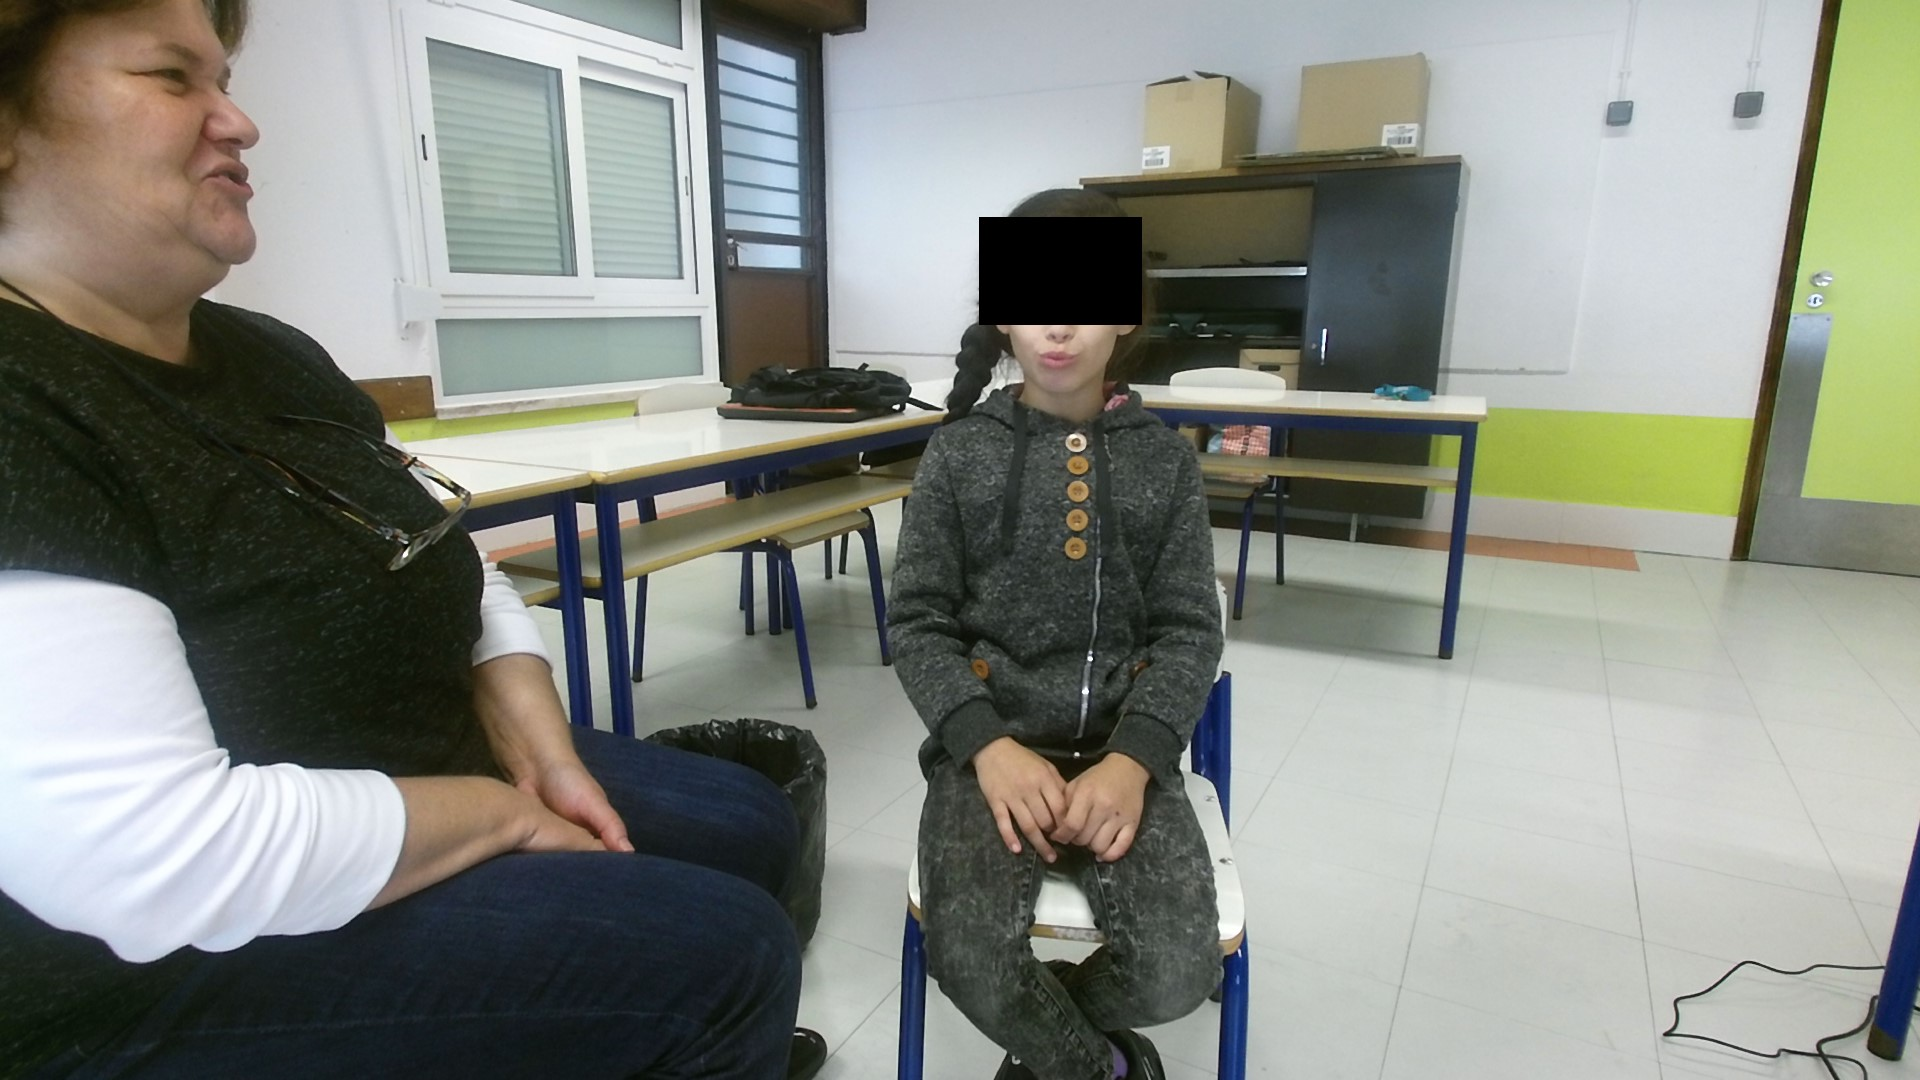
\includegraphics[trim=24cm 16cm 19cm 5cm, clip,width=0.2\linewidth]{color_208}}
\caption{Sequence of protrusion and lips over teeth.}
\label{fig:recordedSeq}
\end{figure}


\subsection{Creation of own Dataset}
\label{subsec:newData}
With the support of the experts mentioned, experimental protocols will be designed to collect data, e.g., from stutterers as well as from health subjects as control group. The goal is to create an experimental protocol which can easily be reproduced. For this purpose the indication of the exercises should be recorded or come from an computerized assistant which is displayed on a monitor to facilitate labeling of the data. After each exercise the subject will be asked to give feedback on his emotional state by filling in a questionnaire. Data will be recorded using a combination of the devices shown in \ref{sec:sensorsFeatures}. Stuttering occurrence as well as prolongations can be labeled manually also by non-experts.

To have data over a longer period of time, subjects could be accompanied during their therapies. For the stuttering case it can be justified to monitor the progress of a stuttering therapy supported by emotional biofeedback. For that purpose two groups would be recorded. Subjects of the first group, would perform the exercises without emotional biofeedback and the second group with. After each exercise the subject would provide feedback on their emotional state. 


%--------------------------------------------------------
\begin{comment}
\section{Available APIs for face analysis}

\textbf{FDNA:} 
Quote: "We use facial analysis, deep learning and artificial intelligence to transform big data into actionable genomic intelligence to improve diagnostics and therapeutics. With the world’s largest network of clinicians, labs and researchers creating one of the fastest growing and most comprehensive genomic databases, FDNA is changing the game for rare disease patients."
\url{http://www.fdna.com}\\


\textbf{OpenFace:}
Quote:OpenFace is a Python and Torch implementation of face recognition with deep neural networks and is based on the CVPR 2015 paper FaceNet: A Unified Embedding for Face Recognition and Clustering by Florian Schroff, Dmitry Kalenichenko, and James Philbin at Google. Torch allows the network to be executed on a CPU or with CUDA. Freely available. \url{https://cmusatyalab.github.io/openface/}\\

\textbf{IMOTIONS:} combines Emotient face expression technology with other physiological signals such EEG, eye tracking, Galvanic Skin response, etc. to improve emotion recognition accuracy
\url{https://imotions.com/emotient/}\\

\textbf{EmoVu:} Deep learning based emotion recognition software that reads facial micro expressions. Uses CNNs, Challenging covariate factors such as pose and lighting variations are mitigated by employing robust face tracking, pose normalization and synthesis, and local lighting invariant feature descriptors. Misclassification is minimized through a rigorous classification scheme comprised of decision rule/filtering, classification, and verification stages. Our classifiers are trained on a large and diverse corpus of images to account for variations in appearance across different settings. Free trial available.
\url{http://emovu.com/e/developers/api/} \\

\textbf{Kairos:} "Provides an API for analyzing facial expressions and fea- tures for emotion recognition, gender and age detection and at- tention management. (Have key for free version)"\url{https://www.kairos.com}\\

\textbf{Project Oxford:} by Microsoft provides APIs for categories such as Vision, Speech, Language, Knowledge and Search. Can be tested for free.
\url{https://azure.microsoft.com/en-us/try/cognitive-services/}\\

\textbf{FaceReader:} by Noldus is widely used for academic purposes. It is a facial expression analysis software for analyzing universal emotions in addition to neutral and contempt. The software is also used to observe gaze direction and head orientation. Used more than 10,000 annotated images for training. Describes the face with 500 key points. Can be rented. 
\url{http://www.noldus.com/human-behavior-research/products/facereader}\\

\textbf{InSight} by Sightcorp is a facial expression analysis API and is also used for eye tracking, age and gender estimation, head pose estimation, etc. 2 weeks free trial.
\url{http://sightcorp.com/insight/}\\
\end{comment}




%--------------------------------------------------------
\section{Sensors and Feature Extraction Algorithms}
\label{sec:sensorsFeatures}

In Fig.~\ref{fig:sensors} an overview of different modalities and corresponding sensors is shown. For each data type, features which can be used for classification are indicated.
OpenFace will be used for face detection. It is a free and open source face recognition with implemented deep neural networks \cite{Amos2016openface}.

OpenSmile is feature extraction tool which permits the extraction of large audio feature spaces in realtime. It combines features from Music Information Retrieval and Speech Processing \url{http://audeering.com/technology/opensmile/}.

Skikit-learn toolbox \url{http://scikit-learn.org/} is written in Python and implements different machine learning classifiers.

\begin{sidewaysfigure}
\centering
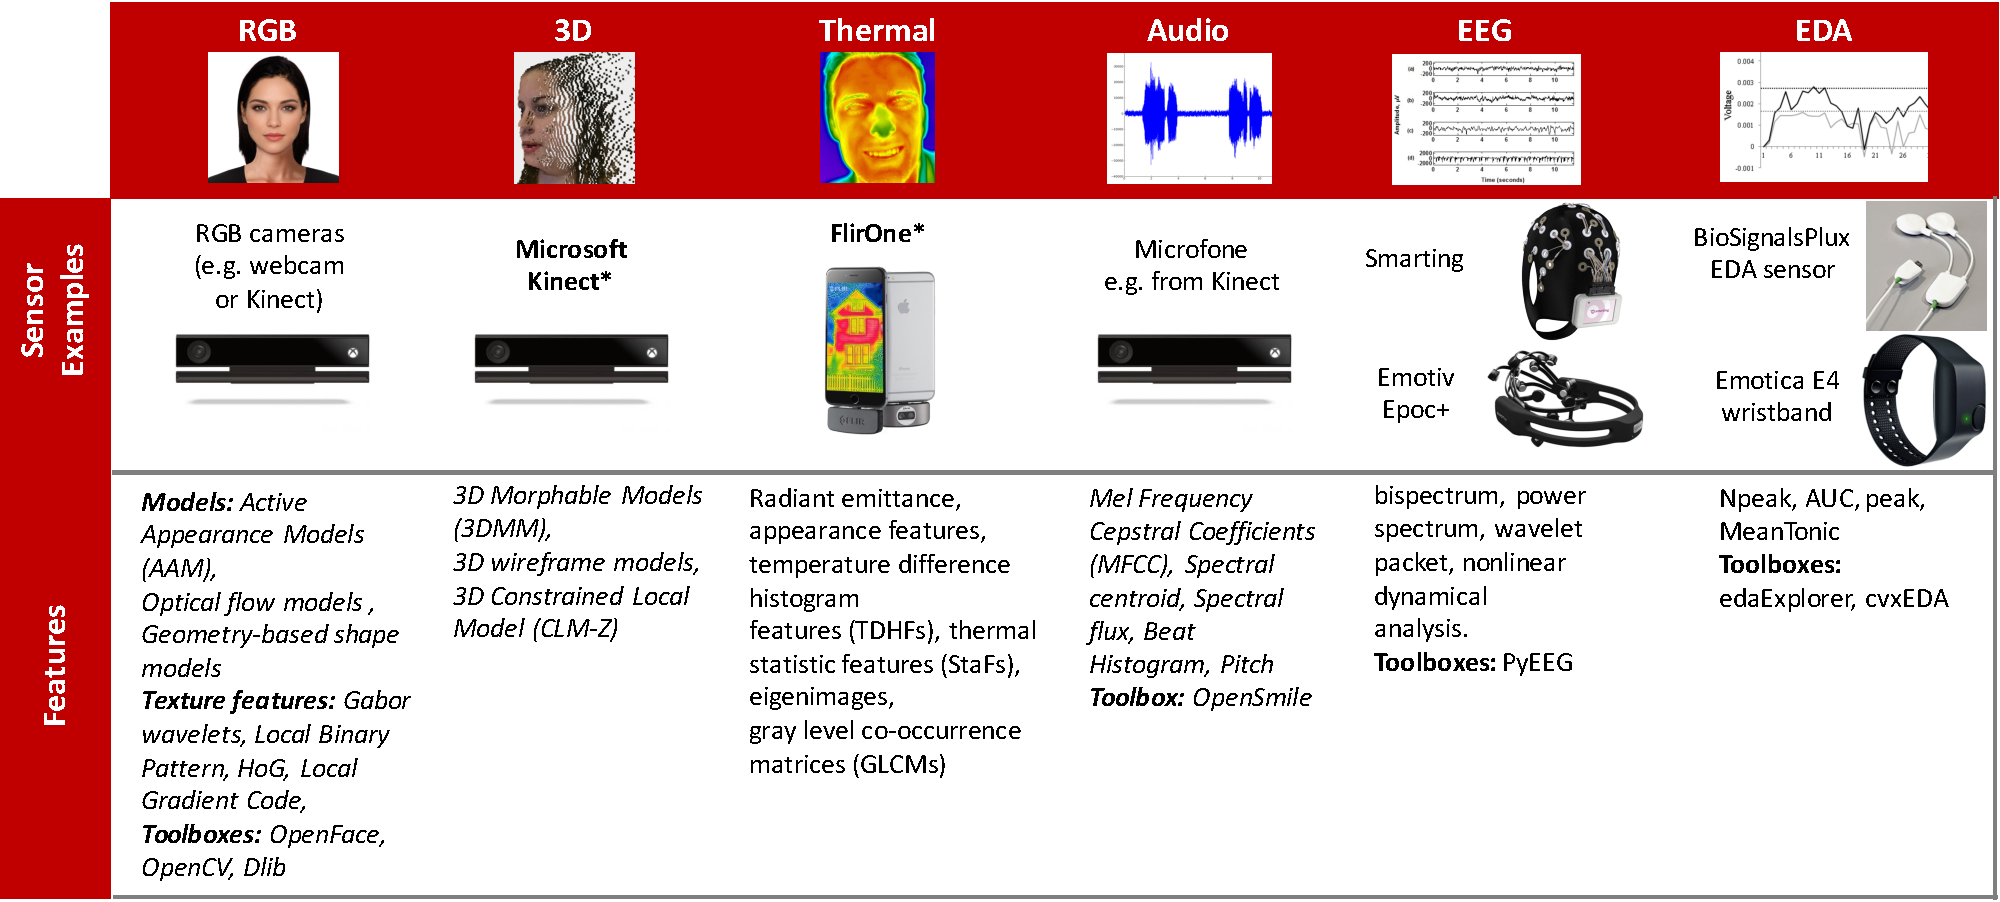
\includegraphics[width=18cm]{methodsSensors}
\caption{Overview of possible sensors to use and of the feature extraction algorithms. * indicates sensors available at the lab.}
\label{fig:sensors}
\end{sidewaysfigure}


\section{Data Fusion}

synchronization of frames, voice and utterance 
